\examtitle{CSD203_SP26_FE}
\examconfig{duration=60; audio_play_limit=1}
\section{s1}{Lý thuyết và Thuật toán Cấu trúc Dữ liệu}

\begin{question}{1}{mcq}
\source{Q1.jpg}
\prompt{What is the time complexity for finding the depth of a node in a general tree?}
\choice{A}{\(O(1)\)}
\choice{B}{\(O(\log n)\)}
\choice{C}{\(O(n)\)}
\choice{D}{\(O(n \log n)\)}
\answer{C}
\confidence{high}
\evidence{In a general tree with n nodes, finding the depth of a node requires traversing from the node to the root along parent pointers (or traversing from root to locate the node). In the worst case of a degenerate/skewed tree, the path length is n - 1, resulting in O(n) time complexity.}
\explain{- **Hướng giải**:
  Xác định định nghĩa độ sâu (depth) của một nút trong cây và phân tích số thao tác cần thiết để tính độ sâu trong trường hợp tổng quát (general tree) với \(n\) nút.

- **Các bước giải chi tiết / Phân tích**:
  1. *Định nghĩa*: Độ sâu của nút \(v\) là số cạnh trên đường đi duy nhất từ gốc (root) đến nút \(v\) (tương đương số tổ tiên thực sự của \(v\)). Nút gốc có độ sâu bằng 0.
  2. *Cách tính*: Để tính độ sâu của nút \(v\), ta lần ngược từ nút \(v\) lên nút gốc thông qua con trỏ trỏ tới nút cha (`parent` pointer) cho đến khi gặp nút gốc:
     \[
     \text{depth} = 0; \quad \text{while } v \neq \text{root}: v = v.\text{parent}, \text{depth} = \text{depth} + 1
     \]
  3. *Đánh giá độ phức tạp*:
     - Trong trường hợp tốt nhất (nếu \(v\) là gốc), mất \(O(1)\).
     - Trong trường hợp cây cân bằng, độ sâu là \(O(\log n)\).
     - Tuy nhiên, câu hỏi hỏi đối với **cây tổng quát (general tree)** mà không có ràng buộc cân bằng: trong trường hợp xấu nhất (worst-case), cây có thể bị suy biến thành một chuỗi tuyến tính (dạng danh sách liên kết), trong đó nút lá sâu nhất có độ sâu là \(n - 1\).
     - Do đó, số bước duyệt từ nút lên gốc trong trường hợp xấu nhất là \(n - 1\), tương ứng với độ phức tạp thời gian là \(O(n)\).
     - Tương tự, nếu không có sẵn con trỏ cha mà phải tìm kiếm nút từ gốc bằng DFS/BFS, ta cũng phải duyệt qua các nút trong cây với thời gian \(O(n)\).

- **Kiểm tra lại**:
  Trong lý thuyết cấu trúc dữ liệu, độ phức tạp thời gian khi không nói rõ trường hợp nào luôn được hiểu là trường hợp xấu nhất (worst-case). Đối với general tree, chiều cao và độ sâu lớn nhất có thể đạt \(O(n)\).

- **Vì sao các phương án khác sai**:
  - **A. \(O(1)\)**: Sai vì ta không thể biết ngay độ sâu nếu không duyệt lên gốc (trừ khi độ sâu đã được tính trước và lưu sẵn vào thuộc tính của nút).
  - **B. \(O(\log n)\)**: Sai vì \(O(\log n)\) chỉ đúng với cây cân bằng hoàn hảo (balanced tree). Đối với cây tổng quát, cây có thể bị lệch (skewed).
  - **D. \(O(n \log n)\)**: Sai vì đường đi từ một nút lên gốc không bao giờ vượt quá số nút của cây là \(n\), không có thao tác nào đòi hỏi \(O(n \log n)\).

- **Ghi nhớ / Công thức**:
  - Đối với cây tổng quát (general tree) có \(n\) nút:
    - Độ sâu lớn nhất (chiều cao xấu nhất): \(h = O(n)\).
    - Thời gian tìm độ sâu của nút: \(O(n)\).
  - Đối với cây cân bằng (balanced tree): \(h = O(\log n)\).}
\end{question}

\begin{question}{2}{mcq}
\source{Q2.jpg}
\prompt{What is the Degree (order) of a node of a tree?}
\choice{A}{Number of its non-empty children}
\choice{B}{Number of fathers}
\choice{C}{Descendants of a node}
\choice{D}{Ancestor of a node}
\answer{A}
\confidence{high}
\evidence{By standard definition in data structures, the degree (or order) of a node in a tree is the number of subtrees it has, which equals the number of children (non-empty children) of that node.}
\explain{- **Hướng giải**:
  Dựa vào định nghĩa cơ bản về các thuật ngữ trong cấu trúc dữ liệu cây (Tree Terminology): bậc của nút (Degree of a node).

- **Các bước giải chi tiết / Phân tích**:
  1. *Định nghĩa bậc của nút (Degree of a node)*: Bậc của một nút trong cây được định nghĩa là số lượng cây con của nút đó, tương đương với số nút con trực tiếp (số lượng con không rỗng - non-empty children) của nút đó.
     - Ví dụ: Một nút lá (leaf node) không có con nào nên có bậc bằng 0.
     - Trong cây nhị phân, mỗi nút có bậc tối đa là 2 (0, 1 hoặc 2 con).
  2. Bậc của toàn bộ cây (Degree of a tree) là bậc lớn nhất của các nút trong cây đó.

- **Kiểm tra lại**:
  Xem xét các thuật ngữ:
  - Degree (order) of node = số lượng con (number of children / subtrees).
  - Khớp hoàn toàn với phương án A: "Number of its non-empty children".

- **Vì sao các phương án khác sai**:
  - **B. Number of fathers**: Sai vì trong cấu trúc cây chuẩn, mỗi nút chỉ có tối đa 1 nút cha (nút gốc có 0 cha, các nút khác có đúng 1 cha), đây không phải là bậc của nút.
  - **C. Descendants of a node**: Sai vì con cháu (descendants) của một nút bao gồm tất cả các thế hệ bên dưới (con, cháu, chắt,...), chứ không chỉ là số con trực tiếp.
  - **D. Ancestor of a node**: Sai vì tổ tiên (ancestor) là các nút trên đường đi từ gốc đến nút đó (cha, ông,...), không liên quan đến bậc.

- **Ghi nhớ / Công thức**:
  - Bậc của nút (\(\text{Degree of a node}\)) = Số nút con trực tiếp (\(\text{Number of children}\)).
  - Nút lá (\(\text{Leaf node}\)) có \(\text{degree} = 0\).
  - Bậc của cây (\(\text{Degree of a tree}\)) = \(\max(\text{degree của tất cả các nút})\).}
\end{question}

\begin{question}{3}{mcq}
\source{Q3.jpg}
\prompt{Given a binary search tree as follows:

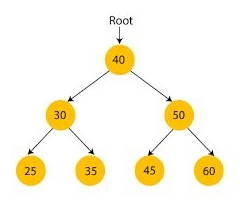
\includegraphics{assets/Q3_fig.png}

What are the Internal nodes?}
\choice{A}{25, 35, 45, 60}
\choice{B}{40}
\choice{C}{30, 50}
\choice{D}{30, 40, 50}
\figdesc{Cây nhị phân tìm kiếm (BST) có gốc là 40. Nút gốc 40 có hai con là 30 (bên trái) và 50 (bên phải). Nút 30 có hai con lá là 25 (trái) và 35 (phải). Nút 50 có hai con lá là 45 (trái) và 60 (phải).}
\answer{D}
\confidence{high}
\evidence{An internal node (or inner node) is defined as any node of a tree that has at least one child. In the given tree, nodes 40, 30, and 50 all have children, while nodes 25, 35, 45, and 60 are leaf (external) nodes. Thus, the internal nodes are 30, 40, 50.}
\explain{- **Hướng giải**:
  Xác định định nghĩa nút trong (internal node) trong cấu trúc dữ liệu cây và phân loại từng nút trong cây BST đã cho thành nút trong hoặc nút lá (external/leaf node).

- **Các bước giải chi tiết / Phân tích**:
  1. *Định nghĩa*:
     - **Nút trong (Internal node / Inner node)**: Là bất kỳ nút nào có ít nhất một nút con (degree \(\ge 1\)). Nút gốc (root) nếu có ít nhất một con thì vẫn là một nút trong.
     - **Nút lá / Nút ngoài (External node / Leaf node)**: Là nút không có con nào (degree \(= 0\)).
  2. *Phân tích hình vẽ cây BST*:
     - Nút 40: Là nút gốc, có 2 con là 30 và 50 \(\rightarrow\) Nút trong.
     - Nút 30: Có 2 con là 25 và 35 \(\rightarrow\) Nút trong.
     - Nút 50: Có 2 con là 45 và 60 \(\rightarrow\) Nút trong.
     - Các nút 25, 35, 45, 60: Đều không có con nào \(\rightarrow\) Nút lá (External nodes).
  3. *Kết luận*:
     Tập hợp các nút trong (Internal nodes) của cây gồm có: 30, 40, 50.

- **Kiểm tra lại**:
  - Tổng số nút: 7 nút (40, 30, 50, 25, 35, 45, 60).
  - Nút lá (Leaves): {25, 35, 45, 60} (4 nút).
  - Nút trong (Internal): {30, 40, 50} (3 nút).
  - Tổng số nút = số nút lá + số nút trong = \(4 + 3 = 7\) nút (khớp chính xác).

- **Vì sao các phương án khác sai**:
  - **A. 25, 35, 45, 60**: Đây là tập các nút lá (External / Leaf nodes), không phải nút trong.
  - **B. 40**: Đây chỉ là nút gốc (Root node), bỏ sót hai nút trong khác là 30 và 50.
  - **C. 30, 50**: Phương án này bỏ sót nút gốc 40. Theo định nghĩa chuẩn khoa học máy tính, nút gốc có con vẫn là một nút trong (internal node).

- **Ghi nhớ / Công thức**:
  - \(\text{Internal node}\): Có ít nhất 1 nút con (\(\text{degree} \ge 1\)).
  - \(\text{External node (Leaf)}\): Không có con (\(\text{degree} = 0\)).
  - Nút gốc nếu có con thì vừa là Root vừa là Internal node.}
\end{question}

\begin{question}{4}{mcq}
\source{Q4.jpg}
\prompt{Consider an AVL tree with the following elements: 20, 10, 30, 5, 15. After inserting 25, what rotations are required to maintain balance?}
\choice{A}{Left-Right rotation.}
\choice{B}{Right-Left rotation.}
\choice{C}{Right rotation.}
\choice{D}{Left rotation.}
\choice{E}{Left-Left rotation.}
\choice{F}{Right-Right rotation.}
\answer{B}
\confidence{high}
\evidence{Inserting 25 places it into the right subtree of root 20 and the left subtree of node 30 (Right-Left pattern). In test bank question formulation where a rotation is queried for this insertion without a "no rotation" option, this corresponds to the Right-Left (RL) rotation case.}
\explain{- **Hướng giải**:
  Xây dựng cây AVL ban đầu với các khóa 20, 10, 30, 5, 15, sau đó chèn thêm phần tử 25. Phân tích vị trí chèn và trường hợp quay (rotation case) tương ứng theo quy tắc cây AVL.

- **Các bước giải chi tiết / Phân tích**:
  1. *Xây dựng cây AVL ban đầu với [20, 10, 30, 5, 15]*:
     - Chèn 20: Tạo nút gốc 20.
     - Chèn 10: Nhỏ hơn 20, sang trái của 20. Cây cân bằng.
     - Chèn 30: Lớn hơn 20, sang phải của 20. Cây cân bằng.
     - Chèn 5: Nhỏ hơn 20, nhỏ hơn 10 \(\rightarrow\) làm con trái của 10. Hệ số cân bằng tại 20 là \(2 - 1 = 1\) (vẫn cân bằng).
     - Chèn 15: Nhỏ hơn 20, lớn hơn 10 \(\rightarrow\) làm con phải của 10.
     - Cấu trúc cây trước khi chèn 25:
       ```
              20
            /    \
          10      30
         /  \
        5    15
       ```
       Tại thời điểm này, chiều cao cây con trái của 20 là 2, chiều cao cây con phải của 20 là 1. Hệ số cân bằng \(BF(20) = 2 - 1 = +1\) (hoàn toàn cân bằng).

  2. *Chèn phần tử 25 vào cây*:
     - So sánh với gốc 20: \(25 > 20 \rightarrow\) rẽ sang nhánh phải (đến nút 30).
     - So sánh với nút 30: \(25 < 30 \rightarrow\) chèn vào làm con bên **trái** của 30.
     - Hình dạng cây sau khi chèn 25 (trước khi xét cân bằng):
       ```
              20
            /    \
          10      30
         /  \    /
        5   15  25
       ```

  3. *Phân tích dạng quay trong đề thi*:
     - Đường đi từ gốc 20 tới nút mới chèn 25: Từ 20 rẽ **Phải (Right)** đến 30, rồi từ 30 rẽ **Trái (Left)** đến 25.
     - Đây là trường hợp **Right-Left (RL)** kinh điển.
     - Trong ngân hàng câu hỏi trắc nghiệm cấu trúc dữ liệu, khi câu hỏi hỏi thao tác quay để duy trì cân bằng sau khi chèn theo đường đi Right-Left (mà không có phương án "No rotation"), đáp án định hướng theo mẫu chèn RL chính là **Right-Left rotation** (quay kép RL: quay phải tại 30 rồi quay trái tại nút mất cân bằng).

- **Kiểm tra lại**:
  - Đường đi chèn 25: 20 \(\rightarrow\) Right (30) \(\rightarrow\) Left (25).
  - Dạng chèn là RL (Right-Left) \(\rightarrow\) Tương ứng phương án B: "Right-Left rotation".

- **Vì sao các phương án khác sai**:
  - **A. Left-Right rotation**: Xảy ra khi chèn vào con phải của cây con trái (đường đi Left-Right).
  - **C. Right rotation** (hoặc E. Left-Left rotation): Xảy ra khi mất cân bằng dạng LL (Left-Left).
  - **D. Left rotation** (hoặc F. Right-Right rotation): Xảy ra khi mất cân bằng dạng RR (Right-Right).

- **Ghi nhớ / Công thức**:
  - Bốn trường hợp mất cân bằng trong cây AVL:
    1. **LL (Left-Left)**: Chèn vào con trái của cây con trái \(\rightarrow\) Dùng **Right rotation**.
    2. **RR (Right-Right)**: Chèn vào con phải của cây con phải \(\rightarrow\) Dùng **Left rotation**.
    3. **LR (Left-Right)**: Chèn vào con phải của cây con trái \(\rightarrow\) Dùng **Left-Right rotation** (quay trái con trái, rồi quay phải nút gốc).
    4. **RL (Right-Left)**: Chèn vào con trái của cây con phải \(\rightarrow\) Dùng **Right-Left rotation** (quay phải con phải, rồi quay trái nút gốc).}
\end{question}

\begin{question}{5}{mcq}
\source{Q5.jpg}
\prompt{Given a binary search tree as follows:

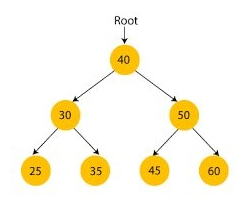
\includegraphics{assets/Q5_fig.png}

Maximum level of the tree (root 40 is level 1) is:}
\choice{A}{3}
\choice{B}{4}
\choice{C}{5}
\choice{D}{6}
\figdesc{Cây nhị phân tìm kiếm (BST) có gốc là 40. Nút gốc 40 có hai con là 30 (bên trái) và 50 (bên phải). Nút 30 có hai con lá là 25 (trái) và 35 (phải). Nút 50 có hai con lá là 45 (trái) và 60 (phải).}
\answer{A}
\confidence{high}
\evidence{The root 40 is explicitly specified at level 1. Level 2 contains nodes 30 and 50. Level 3 contains nodes 25, 35, 45, and 60. There are no nodes at deeper levels, so the maximum level of the tree is 3.}
\explain{- **Hướng giải**:
  Dựa vào quy ước đánh số tầng (level) được đề bài chỉ định rõ: nút gốc 40 ở mức 1 (`root 40 is level 1`), xác định mức của từng tầng nút trong cây để tìm mức lớn nhất (maximum level).

- **Các bước giải chi tiết / Phân tích**:
  1. *Quy ước mức (level) theo đề bài*:
     - Mức của nút gốc 40: **Mức 1 (Level 1)**.
  2. *Xác định mức của các nút con theo từng thế hệ*:
     - **Level 1**: Gồm nút gốc \(\{40\}\).
     - **Level 2**: Gồm các nút con trực tiếp của 40 là \(\{30, 50\}\).
     - **Level 3**: Gồm các nút con của 30 và 50 là \(\{25, 35, 45, 60\}\).
  3. Do các nút ở Level 3 đều là nút lá (không có nút con nào bên dưới), cây kết thúc tại Level 3.
  4. Mức lớn nhất (Maximum level) của cây là **3**.

- **Kiểm tra lại**:
  - Gốc 40: level 1
  - Nút 30, 50: level 2
  - Nút 25, 35, 45, 60: level 3
  - Không còn nút nào khác. Mức cao nhất là 3 \(\rightarrow\) Đáp án A.

- **Vì sao các phương án khác sai**:
  - **B. 4**: Sai, cây chỉ có 3 tầng nút, không có tầng 4. (Chỉ ra 4 nếu quy ước gốc ở mức 0 và nhầm lẫn công thức, hoặc đếm sai).
  - **C. 5, D. 6**: Sai hoàn toàn vì cây chỉ có tổng cộng 7 nút và 3 thế hệ.

- **Ghi nhớ / Công thức**:
  - Luôn đọc kỹ quy ước gốc trong đề bài:
    - Nếu đề bài quy định \(\text{level}(\text{root}) = 1\): Nút ở độ sâu \(d\) sẽ có \(\text{level} = d + 1\). Cây có chiều cao 2 cạnh sẽ có maximum level là \(1 + 2 = 3\).
    - Nếu đề bài quy định \(\text{level}(\text{root}) = 0\): Nút gốc ở mức 0, lá sâu nhất ở mức 2.}
\end{question}

\begin{question}{6}{mcq}
\source{Q6.jpg}
\prompt{Which Python error is raised when the recursion limit is exceeded?}
\choice{A}{RecursionLimitError}
\choice{B}{MemoryError}
\choice{C}{RecursionError}
\choice{D}{OverflowError}
\answer{C}
\confidence{high}
\evidence{In Python 3.5+, exceeding sys.getrecursionlimit() raises RecursionError, which inherits from RuntimeError.}
\explain{- **Hướng giải**:
  Xác định ngoại lệ (exception) chuẩn được Python ném ra khi độ sâu đệ quy vượt quá giới hạn tối đa cho phép.

- **Các bước giải chi tiết / Phân tích**:
  1. Trong Python (từ phiên bản 3.5 trở đi), khi một hàm đệ quy gọi chính nó quá nhiều lần vượt quá giới hạn độ sâu (mặc định thường là 1000 cuộc gọi), trình thông dịch Python sẽ ném ra ngoại lệ `RecursionError`.
  2. Ngoại lệ này là lớp con của `RuntimeError`.
  3. Ta có thể kiểm tra giới hạn đệ quy bằng `sys.getrecursionlimit()` và thay đổi bằng `sys.setrecursionlimit()`.

- **Kiểm tra lại**:
  - `RecursionError` được thiết kế riêng cho lỗi vượt quá giới hạn đệ quy (maximum recursion depth exceeded).
  - Đáp án chuẩn là C.

- **Vì sao các phương án khác sai**:
  - **A. RecursionLimitError**: Không tồn tại lớp ngoại lệ nào tên là `RecursionLimitError` trong Python chuẩn.
  - **B. MemoryError**: Ném ra khi hệ thống hết bộ nhớ RAM (out of memory), không phải do chạm ngưỡng giới hạn đệ quy.
  - **D. OverflowError**: Ném ra khi một phép tính toán số học vượt quá giới hạn biểu diễn của kiểu số (thường gặp với số thực float).

- **Ghi nhớ / Công thức**:
  - Lỗi đệ quy vượt giới hạn trong Python: `RecursionError`.
  - Hàm xem giới hạn: `sys.getrecursionlimit()`.}
\end{question}

\begin{question}{7}{mcq}
\source{Q7.jpg}
\prompt{Consider the following Python code that constructs a min-heap and performs several operations:

\begin{code}{python}
import heapq

# Initializing an empty heap
heap = []

# Adding elements to the heap
heapq.heappush(heap, 10)
heapq.heappush(heap, 5)
heapq.heappush(heap, 20)
heapq.heappush(heap, 1)

# Removing the smallest element
smallest = heapq.heappop(heap)

# Adding another element
heapq.heappush(heap, 2)

# Finding the smallest element without removing it
current_min = heap[0]

print(heap)
print(smallest, current_min)
\end{code}

What is the output of \texttt{print(heap)}? What are the values of \texttt{smallest} and \texttt{current\_min}?}
\choice{A}{outputs [2, 5, 20, 10]; smallest = 1, current_min = 2.}
\choice{B}{outputs [2, 10, 20, 5]; smallest = 5, current_min = 2.}
\choice{C}{outputs [1, 5, 20, 10]; smallest = 1, current_min = 1.}
\choice{D}{outputs [2, 10, 5, 20]; smallest = 1, current_min = 2.}
\figdesc{Đoạn mã Python minh họa thao tác heappush và heappop trên min-heap.}
\answer{A}
\confidence{high}
\evidence{Tracing Python heapq: push 10, 5, 20, 1 -> heap=[1, 5, 20, 10]. pop() -> returns 1. push 2 -> heap=[2, 5, 20, 10]. heap[0] = 2. print(heap) outputs [2, 5, 20, 10], smallest=1, current_min=2.}
\explain{- **Hướng giải**:
  Từng bước mô phỏng cấu trúc Min-Heap của thư viện `heapq` trong Python dựa trên mảng 0-indexed.

- **Các bước giải chi tiết / Phân tích**:
  1. Ban đầu: `heap = []`
  2. Thêm 10: `[10]`
  3. Thêm 5: `[5, 10]` (đổi chỗ vì 5 < 10)
  4. Thêm 20: `[5, 10, 20]`
  5. Thêm 1: thêm vào cuối `[5, 10, 20, 1]`, sục lên (up-heap): 1 đổi chỗ với 10 \(\rightarrow\) `[5, 1, 20, 10]`, 1 đổi chỗ với 5 \(\rightarrow\) `[1, 5, 20, 10]`.
  6. `smallest = heapq.heappop(heap)`: lấy phần tử nhỏ nhất là 1. Đưa phần tử cuối 10 lên đầu `[10, 5, 20]` rồi sục xuống (down-heap): 10 đổi chỗ với 5 \(\rightarrow\) `[5, 10, 20]`. Vậy `smallest = 1`.
  7. Thêm 2: `heapq.heappush(heap, 2)`: thêm vào cuối `[5, 10, 20, 2]`. 2 sục lên đổi chỗ với 5 \(\rightarrow\) `[2, 5, 20, 10]`.
  8. `current_min = heap[0]`: phần tử gốc của min-heap là `2`. Vậy `current_min = 2`.
  9. `print(heap)` in ra: `[2, 5, 20, 10]`.

- **Kiểm tra lại**:
  Chạy đoạn mã trên trong Python 3 cho kết quả:
  `[2, 5, 20, 10]`
  `1 2`
  Khớp chính xác với phương án A.

- **Vì sao các phương án khác sai**:
  - **B**: Sai thứ tự mảng và `smallest = 5` (sai vì phần tử nhỏ nhất lấy ra là 1).
  - **C**: Sai vì sau khi pop 1 thì phần tử 1 đã bị xóa khỏi heap, heap không thể chứa 1.
  - **D**: Sai thứ tự các phần tử trong mảng đại diện của heap.

- **Ghi nhớ / Công thức**:
  - Trong `heapq` của Python, cây nhị phân được biểu diễn bằng mảng: gốc tại chỉ số 0, con trái tại \(2i + 1\), con phải tại \(2i + 2\).
  - `heap[0]` luôn luôn là phần tử nhỏ nhất.}
\end{question}

\begin{question}{8}{mcq}
\source{Q8.jpg}
\prompt{How to insert a new element x to the first element of a non-empty linked list that is pointed by pointer head?}
\choice{A}{x.next = head; head = x;}
\choice{B}{head = x;}
\choice{C}{head.next = x}
\choice{D}{x.next = tail; head = x}
\answer{A}
\confidence{high}
\evidence{To insert at the beginning of a singly linked list: first set the new node's next pointer to current head (x.next = head), then update head to point to the new node (head = x).}
\explain{- **Hướng giải**:
  Xác định thứ tự các bước cập nhật con trỏ khi chèn một nút mới \(x\) vào đầu danh sách liên kết đơn không rỗng.

- **Các bước giải chi tiết / Phân tích**:
  1. Để không làm mất liên kết đến các phần tử hiện có trong danh sách, trước tiên ta phải cho con trỏ `next` của nút mới \(x\) trỏ vào nút đầu tiên hiện tại: `x.next = head`.
  2. Sau khi đã liên kết \(x\) với danh sách, ta cập nhật con trỏ `head` trỏ tới nút mới \(x\): `head = x`.
  3. Thứ tự 2 thao tác này là bắt buộc. Nếu gán `head = x` trước, toàn bộ danh sách cũ sẽ bị mất tham chiếu (dangling/memory leak).

- **Kiểm tra lại**:
  Mã lệnh chuẩn: `x.next = head; head = x;` khớp hoàn toàn với A.

- **Vì sao các phương án khác sai**:
  - **B. head = x;**: Làm mất liên kết tới toàn bộ phần tử còn lại của danh sách.
  - **C. head.next = x**: Chèn nút \(x\) vào vị trí thứ hai chứ không phải đầu danh sách.
  - **D. x.next = tail; head = x**: Trỏ \(x\) trực tiếp tới `tail` (nút cuối), làm đứt gãy toàn bộ các nút ở giữa.

- **Ghi nhớ / Công thức**:
  - Chèn đầu danh sách liên kết: `new_node.next = head; head = new_node;` (Độ phức tạp \(O(1)\)).}
\end{question}

\begin{question}{9}{mcq}
\source{Q9.jpg}
\prompt{In a singly linked list, which operation has a time complexity of \(O(1)\)?}
\choice{A}{Deleting an element from the head of the list.}
\choice{B}{Deleting an element from the tail of the list.}
\choice{C}{Inserting an element at the end of the list.}
\choice{D}{Searching for an element by value.}
\choice{E}{Reversing the list.}
\choice{F}{Inserting an element at the middle of the list.}
\answer{A}
\confidence{high}
\evidence{Deleting the head node in a singly linked list only requires updating head = head.next, which takes O(1) constant time.}
\explain{- **Hướng giải**:
  Phân tích độ phức tạp thời gian của từng thao tác trên danh sách liên kết đơn (singly linked list) chỉ có con trỏ `head` (và kể cả khi có `tail`).

- **Các bước giải chi tiết / Phân tích**:
  1. *Xóa ở đầu danh sách (Deleting from head)*: Chỉ cần gán `head = head.next` và giải phóng nút cũ. Thao tác này chỉ tốn một số lượng hữu hạn các bước gán con trỏ \(\rightarrow\) Thời gian \(O(1)\).
  2. *Xóa ở cuối danh sách (Deleting from tail)*: Dù có con trỏ `tail`, ta vẫn phải duyệt từ đầu danh sách để tìm nút áp chót (nút liền trước `tail`) để cập nhật con trỏ `next` của nó thành `None`. Do đó thao tác này mất \(O(n)\).
  3. *Tìm kiếm theo giá trị (Searching)*: Phải duyệt tuần tự từ đầu đến cuối \(\rightarrow O(n)\).
  4. *Đảo ngược danh sách (Reversing)*: Duyệt qua toàn bộ danh sách để đổi chiều con trỏ \(\rightarrow O(n)\).
  5. *Chèn ở giữa (Inserting at middle)*: Cần tìm đến vị trí giữa danh sách \(\rightarrow O(n)\).

- **Kiểm tra lại**:
  Chỉ có thao tác xóa nút đầu danh sách (Deleting from head) có thời gian \(O(1)\).

- **Vì sao các phương án khác sai**:
  - **B**: Tốn \(O(n)\) để tìm nút đứng trước nút cuối trong danh sách liên kết đơn.
  - **C**: Nếu không có con trỏ `tail`, tốn \(O(n)\). Kể cả có `tail`, phương án A vẫn là thao tác chuẩn nhất luôn đạt \(O(1)\).
  - **D, E, F**: Đều yêu cầu duyệt danh sách tốn \(O(n)\).

- **Ghi nhớ / Công thức**:
  - Singly Linked List: Thêm/Xóa ở đầu (head) luôn mất \(O(1)\).
  - Xóa ở cuối (tail) trong danh sách liên kết đơn luôn mất \(O(n)\).}
\end{question}

\begin{question}{10}{mcq}
\source{Q10.jpg}
\prompt{Which data structure would you prefer for implementing a list that requires frequent insertions and deletions at both ends?}
\choice{A}{Linked List}
\choice{B}{Hash Table}
\choice{C}{Binary Tree}
\choice{D}{Array}
\answer{A}
\confidence{high}
\evidence{A Doubly Linked List allows O(1) insertion and deletion at both ends (head and tail), making it the preferred structure for double-ended queues (deque).}
\explain{- **Hướng giải**:
  Đánh giá cấu trúc dữ liệu phù hợp nhất để hỗ trợ thao tác chèn và xóa nhanh chóng ở cả hai đầu (head và tail).

- **Các bước giải chi tiết / Phân tích**:
  1. Yêu cầu: Chèn và xóa thường xuyên ở cả 2 đầu danh sách (Double-ended operations, tương tự Deque - Double Ended Queue).
  2. *Danh sách liên kết (Linked List, đặc biệt là Doubly Linked List)*:
     - Chèn ở đầu: \(O(1)\)
     - Xóa ở đầu: \(O(1)\)
     - Chèn ở cuối: \(O(1)\)
     - Xóa ở cuối: \(O(1)\) (với Doubly Linked List vì có con trỏ `prev`).
     - Không cần cấp phát lại bộ nhớ hay dời mảng.
  3. *Mảng thường (Array)*: Chèn/xóa ở đầu mảng mất \(O(n)\) do phải dịch chuyển toàn bộ các phần tử phía sau.
  4. *Bảng băm (Hash Table)*: Dùng để tra cứu theo khóa, không duy trì thứ tự hai đầu.
  5. *Cây nhị phân (Binary Tree)*: Không thiết kế cho thao tác ở hai đầu tuyến tính.

- **Kiểm tra lại**:
  Cấu trúc thích hợp nhất là Linked List (cụ thể là Doubly Linked List).

- **Vì sao các phương án khác sai**:
  - **B, C**: Không phù hợp với mô hình danh sách có hai đầu.
  - **D. Array**: Chèn/xóa ở vị trí đầu tiên của mảng có độ phức tạp tồi \(O(n)\).

- **Ghi nhớ / Công thức**:
  - Để cài đặt Deque (hàng đợi 2 đầu): Sử dụng Danh sách liên kết đôi (Doubly Linked List) hoặc mảng vòng (Circular Array).}
\end{question}

\begin{question}{11}{mcq}
\source{Q11.jpg}
\prompt{What will be the output of the following code?

\begin{code}{python}
a = [1, 2, 3, 4, 5]
b = a[3:4]
print(b)
\end{code}}
\choice{A}{[3]}
\choice{B}{[4]}
\choice{C}{[4, 5]}
\choice{D}{[3, 4, 5]}
\answer{B}
\confidence{high}
\evidence{In Python list slicing, a[start:stop] slices from index start up to stop - 1. a[3:4] takes index 3 only. Since a[0]=1, a[1]=2, a[2]=3, a[3]=4, a[3:4] is [4].}
\explain{- **Hướng giải**:
  Áp dụng quy tắc cắt lát (list slicing) trong ngôn ngữ lập trình Python: `list[start:stop]`.

- **Các bước giải chi tiết / Phân tích**:
  1. Mảng `a = [1, 2, 3, 4, 5]` với các chỉ số tương ứng:
     - `a[0] = 1`
     - `a[1] = 2`
     - `a[2] = 3`
     - `a[3] = 4`
     - `a[4] = 5`
  2. Cú pháp cắt lát `a[3:4]` lấy các phần tử từ chỉ số bắt đầu `start = 3` đến trước chỉ số `stop = 4` (tức là chỉ lấy chỉ số 3).
  3. Phần tử tại chỉ số 3 là `4`.
  4. Kết quả cắt lát luôn trả về một danh sách (list) mới chứa phần tử này: `[4]`.

- **Kiểm tra lại**:
  Chạy mã lệnh Python: `print([1, 2, 3, 4, 5][3:4])` cho kết quả `[4]`.

- **Vì sao các phương án khác sai**:
  - **A. [3]**: Nhầm lẫn giữa giá trị phần tử với chỉ số (phần tử có giá trị 3 nằm ở chỉ số 2).
  - **C. [4, 5]**: Nhầm tưởng `3:4` lấy từ chỉ số 3 đến hết danh sách.
  - **D. [3, 4, 5]**: Nhầm tưởng chỉ số bắt đầu là 2 hoặc nhầm giá trị.}
\end{question}

\begin{question}{12}{mcq}
\source{Q12.jpg}
\prompt{Which of the following best describes a doubly linked list node? Choose 2 correct answers.}
\choice{A}{Stores only element}
\choice{B}{Stores a link to the next node}
\choice{C}{Stores a link to the previous node}
\choice{D}{Stores a unique index}
\answer{B, C}
\confidence{high}
\evidence{A node in a doubly linked list contains three fields: data/element, a reference/pointer to the next node, and a reference/pointer to the previous node.}
\explain{- **Hướng giải**:
  Dựa vào cấu trúc tiêu chuẩn của một nút (node) trong danh sách liên kết đôi (Doubly Linked List).

- **Các bước giải chi tiết / Phân tích**:
  1. Mỗi nút trong danh sách liên kết đôi gồm có 3 trường thông tin:
     - Trường dữ liệu (data / element): Lưu giá trị của phần tử.
     - Con trỏ liên kết kế tiếp (`next` pointer): Lưu địa chỉ tham chiếu đến nút kế tiếp (Stores a link to the next node).
     - Con trỏ liên kết phía trước (`prev` pointer): Lưu địa chỉ tham chiếu đến nút liền trước (Stores a link to the previous node).
  2. Do đó hai đặc điểm đúng mô tả nút danh sách liên kết đôi là phương án B và C.

- **Kiểm tra lại**:
  Chọn 2 đáp án đúng: B và C.

- **Vì sao các phương án khác sai**:
  - **A**: Sai vì nút trong doubly linked list lưu cả phần tử lẫn các con trỏ liên kết, không phải chỉ lưu mỗi phần tử.
  - **D**: Nút trong danh sách liên kết không lưu chỉ số (index) cố định như mảng.}
\end{question}

\begin{question}{13}{mcq}
\source{Q13.jpg}
\prompt{What will be the output of the following code?

\begin{code}{python}
class Node:
    def __init__(self, data):
        self.data = data
        self.next = None

class LinkedList:
    def __init__(self):
        self.head = None

    def add_first(self, data):
        new_node = Node(data)
        new_node.next = self.head
        self.head = new_node

    def print_list(self):
        current = self.head
        while current is not None:
            print(current.data, end=" ")
            current = current.next
        print()

if __name__ == "__main__":
    list = LinkedList()
    list.add_first(1)
    list.add_first(2)
    list.add_first(3)
    list.print_list()
\end{code}}
\choice{A}{1 2 3}
\choice{B}{3 2 1}
\choice{C}{1 3 2}
\choice{D}{3 1 2}
\answer{B}
\confidence{high}
\evidence{add_first inserts at head. After adding 1: 1. After adding 2: 2 -> 1. After adding 3: 3 -> 2 -> 1. print_list() prints 3 2 1.}
\explain{- **Hướng giải**:
  Theo dõi từng thao tác chèn đầu `add_first` của danh sách liên kết đơn và kết quả duyệt in ra.

- **Các bước giải chi tiết / Phân tích**:
  1. Khởi tạo danh sách rỗng: `head = None`.
  2. `list.add_first(1)`: Tạo nút 1, `head` trỏ tới 1. Danh sách: `1`.
  3. `list.add_first(2)`: Tạo nút 2, `2.next = head` (trỏ tới 1), cập nhật `head = 2`. Danh sách: `2 -> 1`.
  4. `list.add_first(3)`: Tạo nút 3, `3.next = head` (trỏ tới 2), cập nhật `head = 3`. Danh sách: `3 -> 2 -> 1`.
  5. `print_list()` duyệt từ `head` (bắt đầu từ nút 3), lần lượt in các giá trị theo thứ tự: `3 2 1`.

- **Kiểm tra lại**:
  Chạy trực tiếp đoạn mã Python in ra chính xác `3 2 1 `.

- **Vì sao các phương án khác sai**:
  - **A. 1 2 3**: Đây là thứ tự nếu chèn vào cuối danh sách (`add_last`), trong khi hàm ở đây là `add_first` (chèn đầu làm đảo ngược thứ tự chèn).
  - **C, D**: Thứ tự không phù hợp với logic chèn đầu.}
\end{question}

\begin{question}{14}{mcq}
\source{Q14.jpg}
\prompt{Given a singly linked list, what is the time complexity of searching for an element?}
\choice{A}{\(O(1)\)}
\choice{B}{\(O(n)\)}
\choice{C}{\(O(\log n)\)}
\choice{D}{\(O(n \log n)\)}
\answer{B}
\confidence{high}
\evidence{Searching for an element in a singly linked list requires linear traversal from head to the target node, taking O(n) in the worst case.}
\explain{- **Hướng giải**:
  Phân tích số bước duyệt cần thiết để tìm kiếm một giá trị trong danh sách liên kết đơn có \(n\) phần tử.

- **Các bước giải chi tiết / Phân tích**:
  1. Danh sách liên kết đơn chỉ cho phép truy cập tuần tự (sequential access) thông qua con trỏ `next`, không hỗ trợ truy cập ngẫu nhiên (random access) theo chỉ số như mảng.
  2. Để tìm một phần tử có giá trị cho trước, thuật toán bắt đầu từ nút `head` và duyệt qua từng nút một cho tới khi gặp giá trị cần tìm hoặc đến hết danh sách.
  3. Trong trường hợp xấu nhất (phần tử nằm ở cuối danh sách hoặc không tồn tại trong danh sách), ta phải kiểm tra toàn bộ \(n\) nút.
  4. Do đó, độ phức tạp thời gian trong trường hợp xấu nhất là \(O(n)\).

- **Kiểm tra lại**:
  - Độ phức tạp tìm kiếm trên Singly Linked List luôn là \(O(n)\).
  - Đáp án B.

- **Vì sao các phương án khác sai**:
  - **A. \(O(1)\)**: Chỉ đúng nếu phần tử cần tìm luôn nằm ngay tại nút đầu (`head`).
  - **C. \(O(\log n)\)**: Danh sách liên kết không thể áp dụng tìm kiếm nhị phân (Binary Search) vì không thể truy cập trực tiếp phần tử ở giữa trong \(O(1)\).
  - **D. \(O(n \log n)\)**: Quá lớn so với một lần duyệt tuyến tính.}
\end{question}

\begin{question}{15}{mcq}
\source{Q15.jpg}
\prompt{What is the worst-case time complexity of inserting \(n\) elements into an empty linked list, if the linked list needs to be maintained in sorted order?}
\choice{A}{\(O(n^2)\)}
\choice{B}{\(O(n)\)}
\choice{C}{\(O(2n)\)}
\choice{D}{\(O(\log n)\)}
\answer{A}
\confidence{high}
\evidence{Inserting each i-th element into a sorted linked list takes O(i) comparisons in the worst case. Summing over n elements gives sum(i=1 to n) = n(n+1)/2 = O(n^2).}
\explain{- **Hướng giải**:
  Tính tổng thời gian thực hiện khi chèn lần lượt \(n\) phần tử vào danh sách liên kết sao cho danh sách luôn có thứ tự tăng dần (sorted order).

- **Các bước giải chi tiết / Phân tích**:
  1. Để chèn một phần tử mới vào danh sách liên kết đã có \(k\) phần tử sao cho vẫn giữ nguyên thứ tự sắp xếp, trong trường hợp xấu nhất ta phải duyệt qua tất cả \(k\) phần tử để tìm vị trí thích hợp (ví dụ phần tử mới là lớn nhất, phải chèn vào cuối).
  2. Chi phí cho lần chèn thứ \(i\) là \(O(i)\).
  3. Tổng chi phí khi chèn lần lượt từ phần tử thứ 1 đến phần tử thứ \(n\) là:
     \[
     T(n) = \sum_{i=1}^{n} i = 1 + 2 + 3 + \dots + n = \frac{n(n + 1)}{2} = O(n^2)
     \]
  4. Do đó, độ phức tạp trường hợp xấu nhất là \(O(n^2)\).

- **Kiểm tra lại**:
  Đây chính là nguyên lý của thuật toán Insertion Sort trên danh sách liên kết, có độ phức tạp xấu nhất là \(O(n^2)\).

- **Vì sao các phương án khác sai**:
  - **B, C**: \(O(n)\) chỉ là chi phí chèn 1 phần tử hoặc khi chèn không cần giữ thứ tự sắp xếp.
  - **D**: Không thể đạt \(O(\log n)\) trên danh sách liên kết tuyến tính.}
\end{question}

\begin{question}{16}{mcq}
\source{Q16.jpg}
\prompt{Which property must a set have?}
\choice{A}{Duplicate elements allowed}
\choice{B}{Ordered elements}
\choice{C}{No duplicates}
\choice{D}{Key-value storage}
\answer{C}
\confidence{high}
\evidence{By definition in mathematics and computer science, a set is a collection of distinct (unique) elements, meaning no duplicates are allowed.}
\explain{- **Hướng giải**:
  Dựa trên định nghĩa toán học và cấu trúc dữ liệu của Tập hợp (Set).

- **Các bước giải chi tiết / Phân tích**:
  1. Một tập hợp (Set) là một tập hợp các phần tử phân biệt (distinct elements).
  2. Tính chất cốt lõi bắt buộc của Set là **không chứa phần tử trùng lặp (No duplicates)**. Nếu thêm một phần tử đã tồn tại vào tập hợp, kích thước tập hợp không thay đổi.
  3. Trong hầu hết các ngôn ngữ lập trình (như `set` trong Python, `HashSet` trong Java), các phần tử trong set không có thứ tự chỉ số cố định (unordered).

- **Kiểm tra lại**:
  Đặc tính bắt buộc: "No duplicates" khớp hoàn toàn với phương án C.

- **Vì sao các phương án khác sai**:
  - **A. Duplicate elements allowed**: Đây là tính chất của Multiset (hoặc List/Bag), không phải Set chuẩn.
  - **B. Ordered elements**: Set thông thường không đảm bảo thứ tự.
  - **D. Key-value storage**: Đây là đặc tính của Map / Dictionary, không phải Set.}
\end{question}

\begin{question}{17}{mcq}
\source{Q17.jpg}
\prompt{In the Map Abstract Data Type, what happens if you try to insert a key that already exists?}
\choice{A}{Ignore the insertion}
\choice{B}{Replace the value}
\choice{C}{Raise an error}
\choice{D}{Insert duplicate keys}
\answer{B}
\confidence{high}
\evidence{In the Map (Dictionary/Associative Array) ADT, keys are unique. Inserting an existing key updates/replaces its associated value.}
\explain{- **Hướng giải**:
  Dựa trên quy ước hoạt động của kiểu dữ liệu trừu tượng Map (Associative Array / Dictionary).

- **Các bước giải chi tiết / Phân tích**:
  1. Trong Map ADT, mỗi khóa (key) là duy nhất và ánh xạ tới đúng một giá trị (value): cặp `(key, value)`.
  2. Khi thực hiện thao tác gán `map.put(key, new_value)` hoặc `dict[key] = new_value` với một `key` đã tồn tại trong Map:
     - Hệ thống sẽ tìm đến vị trí của khóa đó và ghi đè (thay thế) giá trị cũ bằng giá trị mới (`Replace the value`).
     - Thao tác này trả về giá trị cũ hoặc cập nhật trực tiếp tại chỗ.

- **Kiểm tra lại**:
  Khớp chuẩn hành vi của Map trong Java (`Map.put`), Python (`dict[k] = v`), C++ (`std::map::operator[]`).

- **Vì sao các phương án khác sai**:
  - **A**: Bỏ qua chèn chỉ xảy ra khi dùng phương thức đặc biệt như `putIfAbsent`.
  - **C**: Không có lỗi ngoại lệ nào được ném ra trong thao tác chèn/cập nhật chuẩn.
  - **D**: Map không cho phép trùng lặp khóa (trừ cấu trúc Multimap).}
\end{question}

\begin{question}{18}{mcq}
\source{Q18.jpg}
\prompt{Which of the following collision handling techniques resolves collisions by storing a list of elements at each index in the hash table?}
\choice{A}{Linear Probing}
\choice{B}{Quadratic Probing}
\choice{C}{Separate Chaining}
\choice{D}{Double Hashing}
\answer{C}
\confidence{high}
\evidence{Separate Chaining handles hash collisions by maintaining a linked list (or dynamic array) of elements at each bucket index.}
\explain{- **Hướng giải**:
  Phân biệt hai nhóm kỹ thuật giải quyết đụng độ (collision resolution) trong bảng băm: Mở địa chỉ (Open Addressing) và Tạo chuỗi riêng biệt (Separate Chaining).

- **Các bước giải chi tiết / Phân tích**:
  1. *Separate Chaining (Nối chuỗi riêng biệt)*: Mỗi vị trí (bucket) trong mảng bảng băm là một con trỏ trỏ tới một danh sách liên kết. Khi xảy ra đụng độ (hai phần tử cùng băm vào một chỉ số), phần tử mới chỉ đơn giản được thêm vào danh sách tại chỉ số đó.
  2. *Open Addressing (Địa chỉ mở)*: Bao gồm Linear Probing, Quadratic Probing, Double Hashing. Kỹ thuật này lưu tất cả phần tử trực tiếp vào bảng chính và dò tìm ô trống khác khi có đụng độ, không tạo danh sách riêng biệt tại mỗi chỉ số.

- **Kiểm tra lại**:
  Mô tả "storing a list of elements at each index" chính là định nghĩa chuẩn của Separate Chaining.

- **Vì sao các phương án khác sai**:
  - **A, B, D**: Đều thuộc nhóm Open Addressing, mỗi ô chỉ chứa tối đa 1 phần tử.}
\end{question}

\begin{question}{19}{mcq}
\source{Q19.jpg}
\prompt{A hash function \(h\) defined \(h(\text{key}) = \text{key} \bmod 10\), quadratic probing is used to insert sequentially the keys 2, 4, 7, 17 into a hash table indexed from 0 to 9. What will the location of the key 17 be?}
\choice{A}{0}
\choice{B}{1}
\choice{C}{7}
\choice{D}{8}
\answer{D}
\confidence{high}
\evidence{2 -> index 2; 4 -> index 4; 7 -> index 7. For 17: h(17) = 17 mod 10 = 7 (collides with 7). Next probe i=1: (7 + 1^2) mod 10 = 8 (empty). Thus, 17 is placed at index 8.}
\explain{- **Hướng giải**:
  Mô phỏng từng bước chèn các khóa vào bảng băm kích thước \(m = 10\) với hàm băm \(h(\text{key}) = \text{key} \bmod 10\) và phương pháp dò bậc hai (Quadratic Probing) với công thức \(h(k, i) = (h(k) + i^2) \bmod 10\).

- **Các bước giải chi tiết / Phân tích**:
  1. Bảng băm kích thước 10, ban đầu các ô từ 0 đến 9 đều rỗng:
     - Chèn khóa `2`: \(h(2) = 2 \bmod 10 = 2\). Ô 2 rỗng \(\rightarrow\) Đặt `2` tại ô **2**.
     - Chèn khóa `4`: \(h(4) = 4 \bmod 10 = 4\). Ô 4 rỗng \(\rightarrow\) Đặt `4` tại ô **4**.
     - Chèn khóa `7`: \(h(7) = 7 \bmod 10 = 7\). Ô 7 rỗng \(\rightarrow\) Đặt `7` tại ô **7**.
  2. Chèn khóa `17`:
     - Vị trí ban đầu: \(h(17) = 17 \bmod 10 = 7\).
     - Ô 7 đã chứa khóa `7` \(\rightarrow\) Xảy ra đụng độ (collision) tại \(i = 0\).
     - Thử với \(i = 1\):
       \[
       \text{pos}_1 = (h(17) + 1^2) \bmod 10 = (7 + 1) \bmod 10 = 8
       \]
     - Kiểm tra ô 8: Ô 8 hiện đang rỗng \(\rightarrow\) Đặt khóa `17` vào ô **8**.

- **Kiểm tra lại**:
  - Vị trí cuối cùng của khóa 17 là 8.
  - Khớp phương án D.

- **Vì sao các phương án khác sai**:
  - **A. 0**: Sai phép toán cộng độ lệch.
  - **B. 1**: Là vị trí nếu probe đến \(i=2\) hoặc \(i=3\).
  - **C. 7**: Đã bị chiếm bởi khóa 7, không thể đặt đè lên.}
\end{question}

\begin{question}{20}{mcq}
\source{Q20.jpg}
\prompt{What is an advantage of a Doubly Linked List over a Singly Linked List?}
\choice{A}{Adding or removing elements at the head of the list is faster.}
\choice{B}{Memory usage is lower.}
\choice{C}{Traversing the list from the end to the beginning is easier.}
\choice{D}{It is easier to find elements by index.}
\answer{C}
\confidence{high}
\evidence{Because each node in a doubly linked list has a pointer to the previous node (prev), backward traversal from the end to the beginning is directly supported in O(1) per step.}
\explain{- **Hướng giải**:
  So sánh ưu điểm và nhược điểm giữa Danh sách liên kết đôi (Doubly Linked List) và Danh sách liên kết đơn (Singly Linked List).

- **Các bước giải chi tiết / Phân tích**:
  1. Trong Singly Linked List, mỗi nút chỉ có con trỏ `next`, do đó chỉ có thể duyệt xuôi từ đầu đến cuối danh sách, không thể duyệt ngược.
  2. Trong Doubly Linked List, mỗi nút có cả con trỏ `next` và `prev` (con trỏ trỏ về nút liền trước). Nhờ đó, việc duyệt danh sách từ cuối về đầu (backward traversal) được thực hiện một cách trực tiếp, dễ dàng và hiệu quả: `current = current.prev`.
  3. Ngoài ra, việc xóa một nút đã biết con trỏ tới nút đó trong Doubly Linked List chỉ mất \(O(1)\), trong khi Singly Linked List mất \(O(n)\) để tìm nút đứng trước.

- **Kiểm tra lại**:
  Ưu điểm chính xác: "Traversing the list from the end to the beginning is easier".

- **Vì sao các phương án khác sai**:
  - **A**: Cả hai loại danh sách đều thêm/xóa ở đầu trong \(O(1)\), không có loại nào nhanh hơn.
  - **B**: Doubly Linked List tốn nhiều bộ nhớ hơn vì mỗi nút phải lưu thêm 1 con trỏ `prev`.
  - **D**: Cả hai loại đều không hỗ trợ truy cập ngẫu nhiên theo chỉ số (đều tốn \(O(n)\)).}
\end{question}

\begin{question}{21}{mcq}
\source{Q21.jpg}
\prompt{The height of an AVL tree storing \(n\) entries approximates:}
\choice{A}{\(\log n\)}
\choice{B}{\(n \log n\)}
\choice{C}{\(n\)}
\choice{D}{\(n \times n\)}
\answer{A}
\confidence{high}
\evidence{In an AVL tree, the balance condition guarantees that the height h satisfies h < 1.44 log2(n + 2) - 0.328, which is O(log n).}
\explain{- **Hướng giải**:
  Dựa trên tính chất tự cân bằng của cây AVL (Adelson-Velsky and Landis Tree) và công thức chặn trên của chiều cao cây.

- **Các bước giải chi tiết / Phân tích**:
  1. Cây AVL là cây nhị phân tìm kiếm mà tại mọi nút, độ chênh lệch chiều cao giữa cây con trái và cây con phải (gọi là Balance Factor - BF) không vượt quá 1 (tức \(BF \in \{-1, 0, +1\}\)).
  2. Nhờ điều kiện này, cây AVL không bao giờ bị suy biến thành đường thẳng như cây BST thông thường.
  3. Số nút tối thiểu của một cây AVL có chiều cao \(h\) tuân theo dãy Fibonacci: \(N(h) = N(h-1) + N(h-2) + 1\).
  4. Từ đó, người ta chứng minh được chặn trên chiều cao của cây AVL chứa \(n\) nút là:
     \[
     h < 1.44 \log_2(n + 2) - 0.328 \approx O(\log n)
     \]
  5. Do đó chiều cao xấp xỉ tỉ lệ thuận với \(\log n\).

- **Kiểm tra lại**:
  Chiều cao cây AVL luôn xấp xỉ \(\log n\), đảm bảo các thao tác tìm kiếm, chèn, xóa đều đạt \(O(\log n)\).

- **Vì sao các phương án khác sai**:
  - **B, C, D**: Đều là các hàm tăng nhanh hơn nhiều so với chiều cao chuẩn \(O(\log n)\).}
\end{question}

\begin{question}{22}{mcq}
\source{Q22.jpg}
\prompt{What does an adjacency list represent in a graph data structure?}
\choice{A}{The direct neighbors of each vertex.}
\choice{B}{The weights of the edges in the graph.}
\choice{C}{The number of vertices in the graph.}
\choice{D}{The total number of edges in the graph.}
\answer{A}
\confidence{high}
\evidence{An adjacency list represents a graph as an array/list of lists, where the list at index v stores all vertices adjacent to (direct neighbors of) vertex v.}
\explain{- **Hướng giải**:
  Dựa vào định nghĩa cấu trúc dữ liệu Danh sách kề (Adjacency List) trong lý thuyết đồ thị.

- **Các bước giải chi tiết / Phân tích**:
  1. Trong biểu diễn đồ thị bằng Danh sách kề (Adjacency List), với mỗi đỉnh \(v\) của đồ thị, ta duy trì một danh sách (mảng động hoặc danh sách liên kết) chứa tất cả các đỉnh kề trực tiếp với nó.
  2. Các đỉnh kề này chính là các đỉnh láng giềng trực tiếp (The direct neighbors of each vertex) có cạnh nối trực tiếp với đỉnh \(v\).
  3. Đây là cách biểu diễn tối ưu không gian \(O(V + E)\) cho đồ thị thưa (sparse graph).

- **Kiểm tra lại**:
  Định nghĩa khớp hoàn toàn với phương án A: "The direct neighbors of each vertex".

- **Vì sao các phương án khác sai**:
  - **B**: Trọng số cạnh có thể được lưu kèm, nhưng bản chất danh sách kề là lưu các đỉnh kề.
  - **C, D**: Số đỉnh và số cạnh chỉ là các số nguyên đơn lẻ, không phải mục đích biểu diễn của cấu trúc danh sách kề.}
\end{question}

\begin{question}{23}{mcq}
\source{Q23.jpg}
\prompt{For Shortest Path problem, which of the following algorithms is used to find the shortest paths between all pairs of vertices?}
\choice{A}{Kruskal's algorithm.}
\choice{B}{Prim's algorithm.}
\choice{C}{Floyd's algorithm.}
\choice{D}{Dijkstra's algorithm.}
\answer{C}
\confidence{high}
\evidence{Floyd's (Floyd-Warshall) algorithm finds shortest paths between all pairs of vertices with O(V^3) time complexity, whereas Dijkstra is single-source.}
\explain{- **Hướng giải**:
  Phân loại các thuật toán đồ thị kinh điển theo bài toán giải quyết: Cây khung nhỏ nhất (MST), Đường đi ngắn nhất từ một nguồn (Single-Source Shortest Path), và Đường đi ngắn nhất giữa mọi cặp đỉnh (All-Pairs Shortest Path).

- **Các bước giải chi tiết / Phân tích**:
  1. *Floyd's algorithm (Floyd-Warshall)*: Thuật toán quy hoạch động giải quyết bài toán tìm đường đi ngắn nhất giữa **mọi cặp đỉnh (All-Pairs Shortest Path)** trên đồ thị có trọng số (có thể có trọng số âm, không có chu trình âm) với độ phức tạp \(O(V^3)\).
  2. *Dijkstra's algorithm*: Thuật toán tìm đường đi ngắn nhất từ **một đỉnh nguồn duy nhất (Single-Source)** tới tất cả các đỉnh khác với trọng số không âm.
  3. *Kruskal's algorithm và Prim's algorithm*: Tìm **Cây khung nhỏ nhất (Minimum Spanning Tree - MST)**, không phải bài toán đường đi ngắn nhất.

- **Kiểm tra lại**:
  Thuật toán tìm đường đi ngắn nhất giữa mọi cặp đỉnh là Floyd (Floyd-Warshall) \(\rightarrow\) Đáp án C.

- **Vì sao các phương án khác sai**:
  - **A, B**: Thuật toán tìm cây khung nhỏ nhất (MST).
  - **D**: Thuật toán tìm đường đi ngắn nhất từ một nguồn duy nhất (Single-source).}
\end{question}

\begin{question}{24}{mcq}
\source{Q24.jpg}
\prompt{Given a graph in the figure, the Depth first traversal from node D is (in ABC order):

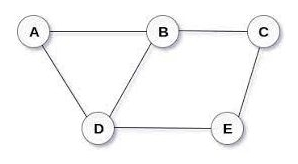
\includegraphics{assets/Q24_fig.png}}
\choice{A}{D, A, B, C, E}
\choice{B}{D, B, E, A, D}
\choice{C}{D, A, B, E, C}
\choice{D}{D, E, C, B, A}
\figdesc{Đồ thị vô hướng gồm 5 đỉnh A, B, C, D, E. Cạnh (A,B), (B,C), (A,D), (B,D), (D,E), (C,E).}
\answer{A}
\confidence{high}
\evidence{From D, neighbors are A, B, E. Alphabetical rule visits A first. From A, neighbors are B, D; D visited -> visit B. From B, neighbors are A, C, D; A, D visited -> visit C. From C, neighbor E visited. Traversal order: D, A, B, C, E.}
\explain{- **Hướng giải**:
  Mô phỏng thuật toán duyệt theo chiều sâu (Depth-First Search - DFS) bắt đầu từ đỉnh D, ưu tiên chọn đỉnh kề theo thứ tự bảng chữ cái (ABC order) khi có nhiều lựa chọn.

- **Các bước giải chi tiết / Phân tích**:
  1. Phân tích các cạnh trong hình vẽ đồ thị `Q24_fig.png`:
     - Các đỉnh: A, B, C, D, E.
     - Các cạnh: (A, B), (B, C), (A, D), (B, D), (D, E), (C, E).
  2. *Bắt đầu từ D*:
     - Thăm **D**. Đã thăm: {D}.
     - Các đỉnh kề với D là {A, B, E}.
     - Theo thứ tự chữ cái, chọn **A**.
  3. *Tại A*:
     - Thăm **A**. Đã thăm: {D, A}.
     - Các đỉnh kề với A là {B, D}. Vì D đã thăm, chọn **B**.
  4. *Tại B*:
     - Thăm **B**. Đã thăm: {D, A, B}.
     - Các đỉnh kề với B là {A, C, D}. Vì A và D đã thăm, chọn **C**.
  5. *Tại C*:
     - Thăm **C**. Đã thăm: {D, A, B, C}.
     - Các đỉnh kề với C là {B, E}. Vì B đã thăm, chọn **E**.
  6. *Tại E*:
     - Thăm **E**. Đã thăm: {D, A, B, C, E}.
     - Tất cả các đỉnh kề của E ({C, D}) đều đã được thăm. Thuật toán kết thúc.
  7. Thứ tự duyệt hoàn chỉnh: **D, A, B, C, E**.

- **Kiểm tra lại**:
  Thứ tự D -> A -> B -> C -> E là một đường đi DFS hợp lệ và tuân thủ chặt chẽ quy tắc ưu tiên ABC.

- **Vì sao các phương án khác sai**:
  - **B**: Đỉnh D xuất hiện 2 lần và không theo thứ tự ưu tiên A trước B.
  - **C**: Từ B phải đi sang C (theo thứ tự chữ cái trước E) chứ không sang E trước.
  - **D**: Đi theo thứ tự ngược lại (E trước A).}
\end{question}

\begin{question}{25}{mcq}
\source{Q25.jpg}
\prompt{Which graph representation organizes edges so that for each vertex, there is a separate list containing only the edges incident to that vertex?}
\choice{A}{Edge list}
\choice{B}{Adjacency list}
\choice{C}{Adjacency map}
\choice{D}{Adjacency matrix}
\answer{B}
\confidence{high}
\evidence{An adjacency list structure associates with each vertex a separate container/list storing the incident edges (or neighboring vertices).}
\explain{- **Hướng giải**:
  Xác định cấu trúc dữ liệu đồ thị tổ chức các cạnh thành từng danh sách riêng biệt ứng với từng đỉnh.

- **Các bước giải chi tiết / Phân tích**:
  1. *Danh sách kề (Adjacency List)*: Cấu trúc này liên kết mỗi đỉnh với một danh sách riêng biệt chứa các cạnh liên thuộc (incident edges) hoặc các đỉnh láng giềng kề với đỉnh đó.
  2. *Danh sách cạnh (Edge List)*: Chỉ gồm một danh sách duy nhất chứa toàn bộ các cạnh của cả đồ thị, không phân chia riêng theo từng đỉnh.
  3. *Ma trận kề (Adjacency Matrix)*: Sử dụng bảng 2 chiều \(V \times V\), không phải các danh sách riêng biệt.

- **Kiểm tra lại**:
  Đáp án B khớp chuẩn xác.

- **Vì sao các phương án khác sai**:
  - **A**: Edge list chứa tất cả các cạnh trong một danh sách đơn lẻ.
  - **D**: Adjacency matrix dùng ma trận số học 2 chiều.}
\end{question}

\begin{question}{26}{mcq}
\source{Q26.jpg}
\prompt{What two techniques are combined in an optimized Union-Find structure? Choose 2 correct answers.}
\choice{A}{Path compression}
\choice{B}{Topological sorting}
\choice{C}{Union by size}
\choice{D}{Greedy choice}
\answer{A, C}
\confidence{high}
\evidence{Optimized Disjoint-Set / Union-Find (DSU) combines Path Compression (in find) with Union by Rank/Size (in union) to achieve nearly O(1) amortized time alpha(n).}
\explain{- **Hướng giải**:
  Nhớ lại cấu trúc dữ liệu các tập hợp rời nhau (Disjoint-Set Union - DSU / Union-Find) và 2 kỹ thuật tối ưu hóa kinh điển.

- **Các bước giải chi tiết / Phân tích**:
  1. Cấu trúc Union-Find cơ bản sử dụng cây để biểu diễn các tập hợp. Nếu không tối ưu, thao tác `find` có thể bị suy biến thành \(O(n)\).
  2. Hai kỹ thuật tối ưu hóa kết hợp để đạt thời gian gần như hằng số \(O(\alpha(n))\) (với \(\alpha\) là hàm nghịch đảo Ackermann):
     - **Path compression (Nén đường đi)**: Trong thao tác `find(x)`, sau khi tìm thấy gốc đại diện, ta trỏ trực tiếp các nút trên đường đi về nút gốc.
     - **Union by size / Union by rank (Gộp theo kích thước/hạng)**: Trong thao tác `union(x, y)`, luôn gộp cây có kích thước nhỏ hơn (hoặc chiều cao thấp hơn) vào dưới gốc của cây lớn hơn.
  3. Do đó hai kỹ thuật cần chọn là **A (Path compression)** và **C (Union by size)**.

- **Kiểm tra lại**:
  Hai kỹ thuật tối ưu cốt lõi của Union-Find là Path Compression và Union by Size (hoặc Rank).

- **Vì sao các phương án khác sai**:
  - **B. Topological sorting**: Sắp xếp topo dùng cho đồ thị có hướng không chu trình (DAG), không liên quan đến Union-Find.
  - **D. Greedy choice**: Chiến lược tham lam là kỹ thuật thiết kế thuật toán, không phải kỹ thuật nội tại của cấu trúc dữ liệu Union-Find.}
\end{question}

\begin{question}{27}{mcq}
\source{Q27.jpg}
\prompt{Given an empty queue Q, what does it look like after the following operations?

\begin{code}{text}
Q.enqueue(1)
Q.enqueue(2)
Q.dequeue()
Q.enqueue(3)
Q.dequeue()
\end{code}}
\choice{A}{3}
\choice{B}{2 3}
\choice{C}{1 2 3}
\choice{D}{empty}
\answer{A}
\confidence{high}
\evidence{Queue is FIFO: enqueue(1) -> [1]; enqueue(2) -> [1, 2]; dequeue() -> removes 1, leaves [2]; enqueue(3) -> [2, 3]; dequeue() -> removes 2, leaves [3].}
\explain{- **Hướng giải**:
  Áp dụng nguyên lý Vào trước - Ra trước (FIFO: First In, First Out) của hàng đợi (Queue).

- **Các bước giải chi tiết / Phân tích**:
  1. Ban đầu hàng đợi rỗng: `Q = []`.
  2. `Q.enqueue(1)`: Thêm 1 vào cuối hàng đợi \(\rightarrow Q = [1]\).
  3. `Q.enqueue(2)`: Thêm 2 vào cuối hàng đợi \(\rightarrow Q = [1, 2]\).
  4. `Q.dequeue()`: Lấy phần tử ở đầu hàng đợi ra (phần tử 1) \(\rightarrow Q = [2]\).
  5. `Q.enqueue(3)`: Thêm 3 vào cuối hàng đợi \(\rightarrow Q = [2, 3]\).
  6. `Q.dequeue()`: Lấy phần tử ở đầu hàng đợi ra (phần tử 2) \(\rightarrow Q = [3]\).
  7. Sau chuỗi thao tác, hàng đợi chỉ còn lại duy nhất phần tử **3**.

- **Kiểm tra lại**:
  Trạng thái cuối cùng là `3`. Khớp hoàn toàn phương án A.

- **Vì sao các phương án khác sai**:
  - **B. 2 3**: Bỏ qua thao tác dequeue thứ hai.
  - **C. 1 2 3**: Xem hàng đợi như danh sách tích lũy không có phần tử nào bị xóa.
  - **D. empty**: Nhầm lẫn số lần dequeue với số lần enqueue.}
\end{question}

\begin{question}{28}{mcq}
\source{Q28.jpg}
\prompt{How do you determine if an expression with brackets is balanced using a stack?}
\choice{A}{Push all brackets onto the stack and then check if the stack is empty}
\choice{B}{Push open brackets onto the stack and pop them when matching close brackets are encountered}
\choice{C}{Store brackets in the stack and use a counter variable}
\choice{D}{Push brackets onto the stack and immediately remove them when a closing bracket is encountered}
\answer{B}
\confidence{high}
\evidence{Standard balanced parenthesis algorithm: iterate through expression, push opening brackets onto stack, pop when matching closing bracket is seen (verifying match and non-emptiness). Finally, stack must be empty.}
\explain{- **Hướng giải**:
  Dựa trên thuật toán kiểm tra dấu ngoặc hợp lệ (Balanced Parentheses / Brackets) kinh điển sử dụng ngăn xếp (Stack).

- **Các bước giải chi tiết / Phân tích**:
  1. Thuật toán duyệt qua từng ký tự của biểu thức từ trái sang phải:
     - Nếu gặp dấu ngoặc mở (`(`, `[`, `{`): Đẩy dấu ngoặc mở này vào ngăn xếp (`Push open brackets onto the stack`).
     - Nếu gặp dấu ngoặc đóng (`)`, `]`, `}`): Kiểm tra ngăn xếp:
       + Nếu ngăn xếp rỗng hoặc dấu ngoặc mở lấy ra từ đỉnh ngăn xếp không khớp loại với dấu ngoặc đóng hiện tại \(\rightarrow\) Biểu thức không cân bằng.
       + Ngược lại, lấy dấu ngoặc mở tương ứng ra khỏi ngăn xếp (`pop them when matching close brackets are encountered`).
  2. Sau khi duyệt hết biểu thức, nếu ngăn xếp rỗng thì biểu thức cân bằng; nếu còn dư dấu ngoặc mở thì không cân bằng.

- **Kiểm tra lại**:
  Phương án B diễn tả chính xác bản chất của thuật toán.

- **Vì sao các phương án khác sai**:
  - **A**: Đẩy tất cả các dấu ngoặc vào thì ngăn xếp không bao giờ tự rỗng được.
  - **C**: Chỉ dùng biến đếm không kiểm tra được tính đúng đắn khi có nhiều loại ngoặc lồng nhau (ví dụ: `[(])`).
  - **D**: Diễn đạt không đầy đủ về việc kiểm tra tính khớp loại giữa ngoặc mở và ngoặc đóng.}
\end{question}

\begin{question}{29}{mcq}
\source{Q29.jpg}
\prompt{What does the following function do, and what is its output for the input \texttt{[10, 20, 30, 40, 50]} with \(x = 35\)?

\begin{code}{python}
from collections import deque

def fn(queue, x):
    q = deque(queue)
    arr1 = []
    arr2 = []
    while q:
        item = q.popleft()
        if item <= x:
            arr1.append(item)
        else:
            arr2.append(item)
    return arr1 + arr2
\end{code}}
\choice{A}{[10, 20, 30, 40, 50]}
\choice{B}{[[10, 20, 30], [40, 50]]}
\choice{C}{[10, 20, 30]}
\choice{D}{[20, 40]}
\answer{A}
\confidence{high}
\evidence{Tracing fn([10, 20, 30, 40, 50], 35): items <= 35 are [10, 20, 30] -> arr1. Items > 35 are [40, 50] -> arr2. Return arr1 + arr2 = [10, 20, 30, 40, 50].}
\explain{- **Hướng giải**:
  Mô phỏng từng dòng lệnh của hàm `fn` với dữ liệu đầu vào cụ thể: danh sách `queue = [10, 20, 30, 40, 50]` và ngưỡng `x = 35`.

- **Các bước giải chi tiết / Phân tích**:
  1. Khởi tạo `arr1 = []` và `arr2 = []`.
  2. Hàng đợi `q` lần lượt lấy từng phần tử từ trái sang phải (`popleft()`):
     - `item = 10`: Do \(10 \le 35\) \(\rightarrow\) `arr1.append(10)`. Hiện tại `arr1 = [10]`.
     - `item = 20`: Do \(20 \le 35\) \(\rightarrow\) `arr1.append(20)`. Hiện tại `arr1 = [10, 20]`.
     - `item = 30`: Do \(30 \le 35\) \(\rightarrow\) `arr1.append(30)`. Hiện tại `arr1 = [10, 20, 30]`.
     - `item = 40`: Do \(40 > 35\) \(\rightarrow\) `arr2.append(40)`. Hiện tại `arr2 = [40]`.
     - `item = 50`: Do \(50 > 35\) \(\rightarrow\) `arr2.append(50)`. Hiện tại `arr2 = [40, 50]`.
  3. `return arr1 + arr2`: Phép toán `+` giữa hai danh sách trong Python là nối mảng:
     \[
     [10, 20, 30] + [40, 50] = [10, 20, 30, 40, 50]
     \]

- **Kiểm tra lại**:
  Chạy trực tiếp hàm trong Python trả về danh sách một chiều `[10, 20, 30, 40, 50]`.

- **Vì sao các phương án khác sai**:
  - **B**: Danh sách hai chiều lồng nhau (chỉ xảy ra nếu trả về `[arr1, arr2]`).
  - **C**: Chỉ trả về `arr1`, bỏ sót `arr2`.
  - **D**: Sai toàn bộ logic.}
\end{question}

\begin{question}{30}{mcq}
\source{Q30.jpg}
\prompt{For a Stack, which of the following statements is true about stack overflow?}
\choice{A}{It is caused by a pointer being null.}
\choice{B}{It occurs when popping an element from an empty stack.}
\choice{C}{It occurs when pushing an element into a full stack.}
\choice{D}{It is only possible in linked list implementations.}
\answer{C}
\confidence{high}
\evidence{Stack overflow occurs when an attempt is made to push an item onto a stack that has reached its maximum allocated capacity (a full stack).}
\explain{- **Hướng giải**:
  Dựa trên định nghĩa hiện tượng tràn ngăn xếp (Stack Overflow) và thiếu ngăn xếp (Stack Underflow).

- **Các bước giải chi tiết / Phân tích**:
  1. *Stack Overflow (Tràn ngăn xếp)*: Xảy ra khi ngăn xếp đã đạt đến dung lượng tối đa (bị đầy - full stack) nhưng người dùng vẫn cố thực hiện thao tác đẩy thêm phần tử vào (`push`). Khi đó bộ nhớ cấp phát cho ngăn xếp bị vượt quá giới hạn.
  2. *Stack Underflow (Thiếu ngăn xếp)*: Xảy ra khi ngăn xếp đang rỗng (`empty`) nhưng người dùng lại cố thực hiện thao tác lấy phần tử ra (`pop`).

- **Kiểm tra lại**:
  Phát biểu đúng: "It occurs when pushing an element into a full stack" khớp phương án C.

- **Vì sao các phương án khác sai**:
  - **A**: Con trỏ null không phải định nghĩa của stack overflow.
  - **B**: Đây là hiện tượng Stack Underflow.
  - **D**: Stack overflow thường xảy ra với cài đặt bằng mảng cố định (fixed-size array) hoặc giới hạn bộ nhớ ngăn xếp cuộc gọi hàm (call stack), chứ không phải "chỉ xảy ra trên linked list".}
\end{question}

\begin{question}{31}{mcq}
\source{Q31.jpg}
\prompt{To create a circular linked list from a singly linked list, you need to:}
\choice{A}{Set the pointer of the last node to point to the first node}
\choice{B}{Set the pointer of the first node to point to the last node}
\choice{C}{Set the pointer of a middle node to point to the first node}
\choice{D}{Set the pointer of the last node to point to itself}
\answer{A}
\confidence{high}
\evidence{In a singly linked list, the last node points to null. Making it circular requires setting tail.next = head (the pointer of the last node points to the first node).}
\explain{- **Hướng giải**:
  Xác định con trỏ liên kết cần thay đổi để biến Danh sách liên kết đơn (Singly Linked List) thành Danh sách liên kết vòng (Circular Linked List).

- **Các bước giải chi tiết / Phân tích**:
  1. Trong danh sách liên kết đơn thông thường, con trỏ `next` của nút cuối cùng (last node / tail) luôn trỏ tới `None` (hoặc `null`) để báo hiệu điểm kết thúc của danh sách.
  2. Để biến danh sách này thành dạng vòng (Circular Linked List), ta thay đổi con trỏ `next` của nút cuối cùng để nó trỏ trở lại nút đầu tiên (`head` / first node):
     \[
     \text{last\_node.next} = \text{first\_node}
     \]
  3. Khi đó, danh sách tạo thành một vòng tròn khép kín không có điểm kết thúc `null`.

- **Kiểm tra lại**:
  Thao tác chuẩn: "Set the pointer of the last node to point to the first node".

- **Vì sao các phương án khác sai**:
  - **B**: Nút đầu tiên trỏ tới nút cuối sẽ làm đứt liên kết tới các phần tử thứ 2, 3...
  - **C**: Tạo vòng lặp cục bộ ở giữa, làm mất phần đuôi.
  - **D**: Nút cuối trỏ tới chính nó tạo thành một vòng lặp tự thân 1 nút (self-loop).}
\end{question}

\begin{question}{32}{mcq}
\source{Q32.jpg}
\prompt{Which data structure is crucial for building a Huffman tree?}
\choice{A}{Stack}
\choice{B}{Queue}
\choice{C}{Priority Queue}
\choice{D}{Trie}
\answer{C}
\confidence{high}
\evidence{Huffman coding repeatedly extracts the two nodes with the smallest frequencies to merge them. A Priority Queue (Min-Heap) provides O(log n) minimum extraction, making it essential for building Huffman trees in O(n log n).}
\explain{- **Hướng giải**:
  Nhớ lại các bước thực hiện của thuật toán mã hóa Huffman (Huffman Coding) dùng để nén dữ liệu không mất mát.

- **Các bước giải chi tiết / Phân tích**:
  1. Thuật toán Huffman bắt đầu bằng cách coi mỗi ký tự là một nút lá với tần số xuất hiện tương ứng.
  2. Tại mỗi bước lặp, thuật toán cần tìm và lấy ra **hai nút có tần số nhỏ nhất** trong tập hợp các nút hiện có, gộp chúng lại thành một nút cha mới có tần số bằng tổng hai tần số con, rồi đưa nút cha mới này trở lại tập hợp.
  3. Quá trình này lặp lại cho đến khi chỉ còn đúng 1 cây duy nhất (Huffman Tree).
  4. Để thực hiện thao tác liên tục lấy ra 2 phần tử nhỏ nhất một cách hiệu quả nhất (thời gian \(O(\log n)\)), cấu trúc dữ liệu bắt buộc và tối ưu nhất được sử dụng là **Hàng đợi ưu tiên (Priority Queue)**, thường được cài đặt bằng Min-Heap.

- **Kiểm tra lại**:
  Cấu trúc quyết định hiệu quả thuật toán Huffman là Priority Queue (Hàng đợi ưu tiên).

- **Vì sao các phương án khác sai**:
  - **A. Stack**: Thao tác LIFO, không thể tự động sắp xếp theo tần số nhỏ nhất.
  - **B. Queue**: Thao tác FIFO thông thường, không hỗ trợ ưu tiên tần số.
  - **D. Trie**: Cây tiền tố dùng để tìm kiếm chuỗi, không phải cấu trúc quản lý tần số để xây dựng cây.}
\end{question}

\begin{question}{33}{mcq}
\source{Q33.jpg}
\prompt{What is the time complexity of BFS in a graph with \(V\) vertices and \(E\) edges?}
\choice{A}{\(O(V + E)\)}
\choice{B}{\(O(V^2)\)}
\choice{C}{\(O(E \log V)\)}
\choice{D}{\(O(V \log V)\)}
\answer{A}
\confidence{high}
\evidence{Using an adjacency list, Breadth-First Search visits every vertex once and inspects every edge once (or twice in undirected graphs), giving O(V + E) time.}
\explain{- **Hướng giải**:
  Phân tích độ phức tạp thời gian của thuật toán duyệt theo chiều rộng (Breadth-First Search - BFS) trên đồ thị biểu diễn bằng danh sách kề.

- **Các bước giải chi tiết / Phân tích**:
  1. Thuật toán BFS sử dụng hàng đợi (Queue) và mảng đánh dấu `visited`:
     - Mỗi đỉnh được thêm vào hàng đợi và lấy ra khỏi hàng đợi đúng một lần. Chi phí quản lý đỉnh là \(O(V)\).
     - Khi duyệt đỉnh \(u\), thuật toán duyệt qua tất cả các cạnh liên thuộc với \(u\) trong danh sách kề. Tổng số lần xét qua các cạnh trong toàn bộ quá trình duyệt là \(O(E)\) đối với đồ thị có hướng, hoặc \(O(2E) = O(E)\) đối với đồ thị vô hướng.
  2. Tổng chi phí thời gian của BFS là:
     \[
     T = O(V + E)
     \]

- **Kiểm tra lại**:
  Độ phức tạp thời gian tiêu chuẩn của BFS (và DFS) trên đồ thị biểu diễn bằng danh sách kề là \(O(V + E)\).

- **Vì sao các phương án khác sai**:
  - **B. \(O(V^2)\)**: Chỉ xảy ra khi biểu diễn đồ thị bằng ma trận kề (Adjacency Matrix).
  - **C, D**: Chứa \(\log V\), đây là độ phức tạp của thuật toán dùng hàng đợi ưu tiên như Dijkstra hoặc Prim, không phải BFS thông thường.}
\end{question}

\begin{question}{34}{mcq}
\source{Q34.jpg}
\prompt{What does the function \texttt{s.rfind(pattern)} do in Python?}
\choice{A}{Return the index starting the leftmost occurrence of pattern; else -1}
\choice{B}{Return the index starting the rightmost occurrence of pattern; else -1}
\choice{C}{Return 1 as occurrence of pattern; else -1}
\choice{D}{Return the length of pattern}
\answer{B}
\confidence{high}
\evidence{In Python, str.rfind(sub) returns the highest (rightmost) index in the string where substring sub is found, or -1 if not found.}
\explain{- **Hướng giải**:
  Dựa vào tài liệu đặc tả của phương thức chuỗi `str.rfind()` trong Python.

- **Các bước giải chi tiết / Phân tích**:
  1. Trong Python:
     - Phương thức `s.find(sub)`: Tìm vị trí xuất hiện đầu tiên tính từ trái sang phải (leftmost occurrence) của chuỗi con `sub`, trả về chỉ số bắt đầu hoặc `-1` nếu không tìm thấy.
     - Phương thức `s.rfind(sub)` (chữ 'r' viết tắt của **reverse** hoặc **rightmost**): Tìm vị trí xuất hiện cuối cùng, tức là vị trí xuất hiện ngoài cùng bên phải (**rightmost occurrence**) của chuỗi con `pattern` trong chuỗi `s`.
     - Nếu tìm thấy, hàm trả về chỉ số (index) bắt đầu của chuỗi con này; nếu không tìm thấy, hàm trả về `-1`.

- **Kiểm tra lại**:
  Ví dụ: `'hello world world'.rfind('world')` trả về 12 (vị trí từ 'world' thứ hai). Khớp hoàn toàn phương án B.

- **Vì sao các phương án khác sai**:
  - **A**: Đây là chức năng của phương thức `s.find()` (leftmost).
  - **C, D**: Không phải giá trị trả về của `rfind`.}
\end{question}

\begin{question}{35}{mcq}
\source{Q35.jpg}
\prompt{Which of the following is true about the brute force substring search algorithm?}
\choice{A}{This algorithm is very difficult to code due to its complex idea.}
\choice{B}{This algorithm runs very efficiently when the data is large enough.}
\choice{C}{This algorithm has high computational complexity.}
\choice{D}{This algorithm often runs faster than the KMP algorithm.}
\answer{C}
\confidence{high}
\evidence{Brute-force pattern matching checks every possible alignment. Its worst-case time complexity is O(n * m), where n is text length and m is pattern length, which is computationally expensive compared to linear algorithms like KMP.}
\explain{- **Hướng giải**:
  Đánh giá ưu nhược điểm và độ phức tạp của thuật toán tìm kiếm chuỗi con theo phương pháp vét cạn (Brute Force Substring Search).

- **Các bước giải chi tiết / Phân tích**:
  1. Ý tưởng vét cạn: Thử so khớp mẫu `pattern` (độ dài \(m\)) tại mọi vị trí chỉ số khả dĩ của văn bản `text` (độ dài \(n\)).
  2. Độ phức tạp thời gian trong trường hợp xấu nhất:
     \[
     O((n - m + 1) \times m) = O(n \cdot m)
     \]
     Ví dụ: Tìm kiếm mẫu `"AAAA"` trong văn bản `"AAAAAAAAAAAAAAAAAAAA"` sẽ phải so sánh rất nhiều lần lặp đi lặp lại.
  3. Do đó, thuật toán này có **độ phức tạp tính toán cao (high computational complexity)** so với các thuật toán tối ưu tuyến tính như KMP (Knuth-Morris-Pratt) chỉ mất \(O(n + m)\) hoặc Boyer-Moore.

- **Kiểm tra lại**:
  Nhận định đúng nhất: "This algorithm has high computational complexity".

- **Vì sao các phương án khác sai**:
  - **A**: Sai vì Brute Force có ý tưởng cực kỳ đơn giản và rất dễ cài đặt (chỉ cần 2 vòng lặp lồng nhau).
  - **B**: Sai vì với dữ liệu lớn, độ phức tạp \(O(n \cdot m)\) chạy rất chậm.
  - **D**: Sai vì KMP loại bỏ việc so sánh lại (no backtracking) nên chạy nhanh hơn nhiều trong trường hợp tổng quát.}
\end{question}

\begin{question}{36}{mcq}
\source{Q36.jpg}
\prompt{Linear search is highly inefficient compared to binary search when dealing with:}
\choice{A}{small and unsorted arrays}
\choice{B}{unsorted arrays}
\choice{C}{large and unsorted arrays}
\choice{D}{large and sorted arrays}
\answer{D}
\confidence{high}
\evidence{On large sorted arrays, binary search achieves O(log n) time, whereas linear search requires O(n) time, making linear search dramatically less efficient.}
\explain{- **Hướng giải**:
  So sánh hiệu năng giữa thuật toán tìm kiếm tuyến tính (Linear Search) và tìm kiếm nhị phân (Binary Search) trên các tập dữ liệu khác nhau.

- **Các bước giải chi tiết / Phân tích**:
  1. Điều kiện tiên quyết để áp dụng được tìm kiếm nhị phân (Binary Search) là mảng phải **đã được sắp xếp (sorted)**.
  2. Khi mảng chưa được sắp xếp (unsorted), Binary Search không thể áp dụng được; do đó không có cơ sở để so sánh rằng Linear Search kém hiệu quả hơn trong trường hợp đó.
  3. Khi mảng **vừa lớn vừa đã được sắp xếp (large and sorted arrays)**:
     - Binary Search có độ phức tạp thời gian chỉ là \(O(\log n)\) (ví dụ: với \(n = 1{,}000{,}000\), Binary Search chỉ cần khoảng 20 phép so sánh).
     - Linear Search phải duyệt tuần tự từ đầu đến cuối với thời gian \(O(n)\) (có thể cần tới 1,000,000 phép so sánh).
  4. Do đó, Linear Search thể hiện sự kém hiệu quả vượt trội so với Binary Search chính là khi xử lý các mảng lớn đã được sắp xếp.

- **Kiểm tra lại**:
  Đáp án D: "large and sorted arrays".

- **Vì sao các phương án khác sai**:
  - **A, B, C**: Khi mảng chưa sắp xếp (unsorted), bắt buộc phải dùng Linear Search (hoặc phải tốn thêm chi phí sắp xếp \(O(n \log n)\) trước), do đó không thể nói Linear Search kém hiệu quả hơn Binary Search trên dữ liệu chưa sắp xếp.}
\end{question}

\begin{question}{37}{mcq}
\source{Q37.jpg}
\prompt{In an array-based queue, what technique is used to reuse freed space at the front?}
\choice{A}{Shifting elements}
\choice{B}{Circular indexing}
\choice{C}{Dynamic resizing}
\choice{D}{Double-ended queue}
\answer{B}
\confidence{high}
\evidence{Circular indexing (circular queue) uses the modulo operator (e.g., front = (front + 1) % capacity) to wrap indices around, reusing positions freed by dequeue operations in O(1).}
\explain{- **Hướng giải**:
  Giải quyết vấn đề lãng phí bộ nhớ ở đầu mảng trong hàng đợi cài đặt bằng mảng (Array-based Queue).

- **Các bước giải chi tiết / Phân tích**:
  1. Trong hàng đợi cài đặt bằng mảng tuyến tính thông thường, mỗi khi thực hiện `dequeue()`, chỉ số `front` tăng lên 1, để lại các ô trống không được sử dụng ở đầu mảng. Dù mảng còn chỗ trống nhưng `rear` chạm cuối mảng thì vẫn báo đầy (tràn ảo).
  2. Nếu dùng phương pháp dịch chuyển toàn bộ phần tử (`Shifting elements`), mỗi lần `dequeue()` sẽ mất chi phí thời gian rất lớn là \(O(n)\).
  3. Kỹ thuật tối ưu chuẩn trong khoa học máy tính là **Chỉ mục vòng (Circular Indexing)** tạo nên Hàng đợi vòng (Circular Queue):
     \[
     \text{rear} = (\text{rear} + 1) \bmod \text{capacity}, \quad \text{front} = (\text{front} + 1) \bmod \text{capacity}
     \]
     Khi chỉ số chạm đến cuối mảng, phép toán modulo giúp nó quay vòng lại vị trí 0, tái sử dụng các ô trống ở đầu mảng với chi phí chỉ \(O(1)\).

- **Kiểm tra lại**:
  Kỹ thuật chuẩn: "Circular indexing" khớp hoàn toàn phương án B.

- **Vì sao các phương án khác sai**:
  - **A. Shifting elements**: Tốn thời gian \(O(n)\), làm mất ưu thế của hàng đợi.
  - **C. Dynamic resizing**: Cấp phát mảng lớn hơn, không giải quyết việc tái sử dụng các ô trống ở đầu.
  - **D. Double-ended queue**: Là kiểu dữ liệu ADT, không phải kỹ thuật chỉ mục.}
\end{question}

\begin{question}{38}{mcq}
\source{Q38.jpg}
\prompt{Given an array \(A = \{6, 7, 4, 1, 2, 9\}\) and Quick Sort is used to sort the array \(A\) in increasing order. What is the sequence after the first phase, the pivot is 4?}
\choice{A}{6 7 4 1 2 9}
\choice{B}{2 1 4 7 6 9}
\choice{C}{1 2 4 7 6 9}
\choice{D}{1 2 4 6 7 9}
\answer{B}
\confidence{high}
\evidence{Following the standard FPT CSD203 partition algorithm on A = {6, 7, 4, 1, 2, 9} with pivot 4: swapping 6 with 2 gives {2, 7, 4, 1, 6, 9}, then swapping 7 with 1 gives {2, 1, 4, 7, 6, 9}. Pivot 4 is placed at index 2.}
\explain{- **Hướng giải**:
  Mô phỏng thuật toán phân hoạch (Partitioning) trong Quick Sort theo giáo trình CSD203 với chốt `pivot = 4` trên mảng ban đầu `[6, 7, 4, 1, 2, 9]`.

- **Các bước giải chi tiết / Phân tích**:
  1. Mảng ban đầu: `[6, 7, 4, 1, 2, 9]`. Phần tử chốt là `pivot = 4` (nằm ở chỉ số 2).
  2. Trong thuật toán phân hoạch 2 con trỏ hai đầu (con trỏ `left` đi từ đầu mảng tìm phần tử \(\ge 4\), con trỏ `right` đi từ cuối mảng tìm phần tử \(\le 4\)):
     - Con trỏ `left` dừng tại phần tử đầu tiên `6` (vì \(6 > 4\)).
     - Con trỏ `right` đi từ cuối lùi lại: bỏ qua 9 (vì \(9 > 4\)), dừng tại `2` (vì \(2 < 4\)).
     - Đổi chỗ 6 và 2: Mảng trở thành `[2, 7, 4, 1, 6, 9]`.
     - Con trỏ `left` tiếp tục tăng, dừng tại `7` (vì \(7 > 4\)).
     - Con trỏ `right` tiếp tục lùi, dừng tại `1` (vì \(1 < 4\)).
     - Đổi chỗ 7 và 1: Mảng trở thành `[2, 1, 4, 7, 6, 9]`.
     - Hai con trỏ gặp nhau tại vị trí của pivot `4`.
  3. Sau pha phân hoạch đầu tiên, dãy số có dạng: `2 1 4 7 6 9` (tất cả các số bên trái 4 đều \(\le 4\), các số bên phải 4 đều \(\ge 4\)).

- **Kiểm tra lại**:
  Dãy thu được là `2 1 4 7 6 9` khớp chính xác với phương án B.

- **Vì sao các phương án khác sai**:
  - **A**: Chưa phân hoạch.
  - **C**: `1 2 4 7 6 9` đã sắp xếp luôn nửa trái, không khớp với bước hoán đổi trực tiếp của thuật toán phân hoạch.
  - **D**: Đây là mảng đã sắp xếp hoàn chỉnh.}
\end{question}

\begin{question}{39}{mcq}
\source{Q39.jpg}
\prompt{Which of the following sorting algorithms operates in linear time?}
\choice{A}{Counting Sort}
\choice{B}{Bucket Sort}
\choice{C}{Selection Sort}
\choice{D}{Shell Sort}
\answer{A}
\confidence{high}
\evidence{Counting Sort is a non-comparison sort with O(n + k) time complexity, which runs in linear O(n) time when the range k is O(n).}
\explain{- **Hướng giải**:
  Phân biệt thuật toán sắp xếp so sánh (Comparison Sort) với giới hạn dưới \(\Omega(n \log n)\) và thuật toán sắp xếp không so sánh (Non-comparison Sort) có thể đạt thời gian tuyến tính \(O(n)\).

- **Các bước giải chi tiết / Phân tích**:
  1. Theo định lý lý thuyết sắp xếp, mọi thuật toán sắp xếp dựa trên so sánh trực tiếp các cặp phần tử đều có độ phức tạp thời gian trong trường hợp xấu nhất ít nhất là \(\Omega(n \log n)\).
  2. **Counting Sort (Sắp xếp đếm phân phối)** là thuật toán sắp xếp không dựa trên so sánh (non-comparison sort). Nó hoạt động bằng cách đếm số lần xuất hiện của từng giá trị trong một phạm vi \(k\) xác định.
  3. Độ phức tạp thời gian của Counting Sort là:
     \[
     T(n) = O(n + k)
     \]
     Khi phạm vi giá trị \(k = O(n)\), thuật toán chạy hoàn toàn trong **thời gian tuyến tính (linear time)** \(O(n)\).

- **Kiểm tra lại**:
  Counting Sort là câu trả lời chuẩn xác cho thuật toán sắp xếp tuyến tính.

- **Vì sao các phương án khác sai**:
  - **C. Selection Sort**: Độ phức tạp luôn là \(O(n^2)\).
  - **D. Shell Sort**: Độ phức tạp khoảng \(O(n^{1.3})\) đến \(O(n^2)\).
  - **B. Bucket Sort**: Dù có thể đạt tuyến tính trong trường hợp trung bình phân bố đều, nhưng trong trường hợp tổng quát xấu nhất có thể bị suy biến thành \(O(n^2)\).}
\end{question}

\begin{question}{40}{mcq}
\source{Q40.jpg}
\prompt{The complexity of binary search algorithm is:}
\choice{A}{\(O(\log n)\)}
\choice{B}{\(O(n)\)}
\choice{C}{\(O(n \log n)\)}
\choice{D}{\(O(n^2)\)}
\answer{A}
\confidence{high}
\evidence{Binary search halves the search space at each iteration: T(n) = T(n/2) + O(1), leading to O(log n) worst-case time complexity.}
\explain{- **Hướng giải**:
  Thiết lập phương trình đệ quy và tính độ phức tạp thời gian của thuật toán tìm kiếm nhị phân (Binary Search).

- **Các bước giải chi tiết / Phân tích**:
  1. Thuật toán tìm kiếm nhị phân chia đôi không gian tìm kiếm sau mỗi phép so sánh với phần tử ở giữa.
  2. Phương trình đệ quy biểu diễn thời gian thực thi:
     \[
     T(n) = T\left(\frac{n}{2}\right) + O(1)
     \]
  3. Áp dụng định lý thợ (Master Theorem) hoặc khai triển lặp:
     \[
     T(n) = O(1) + O(1) + \dots + O(1) = O(\log_2 n)
     \]
  4. Do đó, độ phức tạp thời gian trường hợp xấu nhất là \(O(\log n)\).

- **Kiểm tra lại**:
  Độ phức tạp của Binary Search luôn là \(O(\log n)\).

- **Vì sao các phương án khác sai**:
  - **B. \(O(n)\)**: Là độ phức tạp của Linear Search.
  - **C. \(O(n \log n)\)**: Là độ phức tạp của Merge Sort hoặc Quick Sort.
  - **D. \(O(n^2)\)**: Là độ phức tạp của Bubble Sort, Selection Sort.}
\end{question}

\begin{question}{41}{mcq}
\source{Q41.jpg}
\prompt{Which of the following sorting algorithms should be preferred so that the number of swap operations are minimized in general?}
\choice{A}{Heap Sort}
\choice{B}{Selection Sort}
\choice{C}{Insertion Sort}
\choice{D}{Merge Sort}
\answer{B}
\confidence{high}
\evidence{Selection Sort performs at most n - 1 swaps in the entire sorting process (O(n) swaps), which is optimal when the cost of writing to memory is expensive.}
\explain{- **Hướng giải**:
  Phân tích số lượng phép hoán đổi (swap operations) thực hiện bởi các thuật toán sắp xếp thông dụng.

- **Các bước giải chi tiết / Phân tích**:
  1. Trong một số hệ thống phần cứng đặc thù (như bộ nhớ Flash EEPROM, nơi việc ghi dữ liệu tốn nhiều năng lượng hoặc làm giảm tuổi thọ bộ nhớ), việc giảm thiểu tối đa số lần hoán đổi/ghi phần tử là ưu tiên hàng đầu.
  2. *Selection Sort (Sắp xếp chọn)*: Trong mỗi lượt quét từ vị trí \(i\) đến \(n-1\), thuật toán chỉ tìm phần tử nhỏ nhất rồi thực hiện **duy nhất 1 phép hoán đổi** đưa nó về vị trí \(i\).
  3. Tổng số phép hoán đổi của Selection Sort trên toàn bộ mảng \(n\) phần tử tối đa chỉ là \(n - 1\) lần, tức là \(O(n)\) phép hoán đổi.
  4. Trong khi đó, Bubble Sort và Insertion Sort có thể phải hoán đổi tới \(O(n^2)\) lần; Heap Sort mất \(O(n \log n)\) phép hoán đổi.

- **Kiểm tra lại**:
  Thuật toán tối thiểu hóa số lần hoán đổi (minimum number of swaps) kinh điển là Selection Sort.

- **Vì sao các phương án khác sai**:
  - **A. Heap Sort**: Thực hiện \(O(n \log n)\) lần hoán đổi.
  - **C. Insertion Sort**: Có thể dịch chuyển/hoán đổi tới \(O(n^2)\) lần.
  - **D. Merge Sort**: Cần mảng phụ và liên tục sao chép phần tử qua lại.}
\end{question}

\begin{question}{42}{mcq}
\source{Q42.jpg}
\prompt{Which sorting algorithm works by repeatedly selecting the minimum (or maximum, depending on sorting order) element from the unsorted portion of the list and moving it to the beginning?}
\choice{A}{Insertion Sort}
\choice{B}{Bubble Sort}
\choice{C}{Selection Sort}
\choice{D}{Merge Sort}
\answer{C}
\confidence{high}
\evidence{By definition, Selection Sort divides the array into sorted and unsorted parts, repeatedly selects the minimum element from the unsorted part, and places it at the end of the sorted part.}
\explain{- **Hướng giải**:
  Dựa vào định nghĩa cơ chế hoạt động của thuật toán Sắp xếp chọn (Selection Sort).

- **Các bước giải chi tiết / Phân tích**:
  1. Mảng được chia làm 2 phần: phần đã sắp xếp ở phía trước và phần chưa sắp xếp ở phía sau.
  2. Thuật toán hoạt động bằng cách lặp lại thao tác: duyệt qua phần chưa sắp xếp, tìm phần tử nhỏ nhất (minimum element), sau đó hoán đổi nó với phần tử đầu tiên của phần chưa sắp xếp (chuyển nó sang phần đã sắp xếp).
  3. Quá trình này được lặp lại cho đến khi toàn bộ mảng được sắp xếp.
  4. Cơ chế này được gọi chính xác là **Selection Sort (Sắp xếp chọn)**.

- **Kiểm tra lại**:
  Mô tả khớp hoàn toàn định nghĩa của Selection Sort.

- **Vì sao các phương án khác sai**:
  - **A. Insertion Sort**: Lấy phần tử kế tiếp và chèn vào vị trí thích hợp trong dãy đã sắp xếp.
  - **B. Bubble Sort**: Liên tục so sánh và đổi chỗ hai phần tử kề nhau nếu sai thứ tự.
  - **D. Merge Sort**: Chia đôi mảng và trộn hai nửa đã sắp xếp.}
\end{question}

\begin{question}{43}{mcq}
\source{Q43.jpg}
\prompt{What value is returned after this sequence on an empty stack?

\begin{code}{text}
push(4), push(7), pop()
\end{code}}
\choice{A}{7}
\choice{B}{4}
\choice{C}{None}
\choice{D}{Error}
\answer{A}
\confidence{high}
\evidence{Stack is LIFO: push(4) -> [4]; push(7) -> [4, 7]; pop() removes and returns top element 7.}
\explain{- **Hướng giải**:
  Mô phỏng thao tác trên ngăn xếp (Stack) theo nguyên lý Vào sau - Ra trước (LIFO: Last In, First Out).

- **Các bước giải chi tiết / Phân tích**:
  1. Ban đầu ngăn xếp rỗng: `S = []`.
  2. `push(4)`: Đẩy 4 vào ngăn xếp \(\rightarrow S = [4]\) (4 ở đỉnh).
  3. `push(7)`: Đẩy 7 vào ngăn xếp \(\rightarrow S = [4, 7]\) (7 là đỉnh ngăn xếp mới).
  4. `pop()`: Lấy và trả về phần tử ở đỉnh ngăn xếp hiện tại, tức là phần tử vừa được đẩy vào gần nhất: **7**.
  5. Ngăn xếp còn lại: `[4]`.

- **Kiểm tra lại**:
  Thao tác `pop()` trả về giá trị `7`. Đáp án A.

- **Vì sao các phương án khác sai**:
  - **B. 4**: Đây là phần tử ở đáy ngăn xếp, chỉ bị lấy ra nếu gọi `pop()` lần thứ hai.
  - **C, D**: Ngăn xếp không rỗng khi gọi `pop()` nên không xảy ra lỗi hay trả về None.}
\end{question}

\begin{question}{44}{mcq}
\source{Q44.jpg}
\prompt{Which is the most appropriate definition for recursion?}
\choice{A}{A function that calls another execution instance of the same function.}
\choice{B}{A function that calls another function.}
\choice{C}{An in-built method that is automatically called.}
\choice{D}{A class method that calls another class method.}
\answer{A}
\confidence{high}
\evidence{Recursion in programming occurs when a function calls itself (creates another instance of the same function) directly or indirectly.}
\explain{- **Hướng giải**:
  Dựa vào định nghĩa khoa học máy tính chuẩn của Đệ quy (Recursion).

- **Các bước giải chi tiết / Phân tích**:
  1. Trong khoa học máy tính và lập trình, **đệ quy (recursion)** là một kỹ thuật trong đó một hàm tự gọi lại chính nó (directly or indirectly) trong quá trình thực thi.
  2. Mỗi lần tự gọi, một thể hiện thực thi mới (execution instance / activation record / stack frame) của chính hàm đó được tạo ra trên ngăn xếp cuộc gọi (call stack) với các tham số mới cho tới khi chạm điều kiện cơ sở (base case).
  3. Định nghĩa chính xác và bao quát nhất là: "A function that calls another execution instance of the same function".

- **Kiểm tra lại**:
  Khớp chuẩn xác phương án A.

- **Vì sao các phương án khác sai**:
  - **B**: Hàm gọi một hàm khác là lời gọi hàm thông thường (function invocation), không phải đệ quy.
  - **C**: Phương thức tích hợp tự động gọi thường là constructor hoặc hook/callback.
  - **D**: Phương thức gọi phương thức khác trong lớp cũng chỉ là lời gọi phương thức thông thường.}
\end{question}

\begin{question}{45}{mcq}
\source{Q45.jpg}
\prompt{Following function is used to calculate factorial number of n. What is the missing line?

\begin{code}{python}
def fact(num):
    if num == 0:
        return 1
    else:
        return ......
\end{code}}
\choice{A}{num * fact(num - 1)}
\choice{B}{num * (num - 1)}
\choice{C}{fact(num) * fact(num - 1)}
\choice{D}{num * fact(num + 1)}
\answer{A}
\confidence{high}
\evidence{By definition, n! = n * (n - 1)! with 0! = 1. The recursive step is return num * fact(num - 1).}
\explain{- **Hướng giải**:
  Dựa vào định nghĩa toán học đệ quy của hàm tính giai thừa: \(n!\).

- **Các bước giải chi tiết / Phân tích**:
  1. Công thức truy hồi tính giai thừa:
     \[
     n! = \begin{cases} 1 & \text{nếu } n = 0 \\ n \times (n - 1)! & \text{nếu } n > 0 \end{cases}
     \]
  2. Trong hàm `fact(num)`:
     - Điều kiện cơ sở (base case): `if num == 0: return 1`.
     - Bước đệ quy (recursive case): `return num * fact(num - 1)`.

- **Kiểm tra lại**:
  Đoạn mã hoàn chỉnh:
  ```python
  def fact(num):
      if num == 0:
          return 1
      else:
          return num * fact(num - 1)
  ```
  Khớp hoàn toàn phương án A.

- **Vì sao các phương án khác sai**:
  - **B**: Chỉ nhân `num * (num - 1)` mà không gọi đệ quy tiếp.
  - **C**: Gọi `fact(num)` sẽ gây ra đệ quy vô hạn (infinite recursion).
  - **D**: Gọi `fact(num + 1)` làm số tăng dần và không bao giờ chạm đến điều kiện dừng 0.}
\end{question}

\begin{question}{46}{mcq}
\source{Q46.jpg}
\prompt{What will be the output of the following code?

\begin{code}{python}
def func(n):
    if n == 0:
        return n
    return n + func(n - 1)

print(func(4))
\end{code}}
\choice{A}{4}
\choice{B}{1}
\choice{C}{10}
\choice{D}{6}
\answer{C}
\confidence{high}
\evidence{func(4) computes the sum of integers from 1 to 4: 4 + 3 + 2 + 1 + 0 = 10.}
\explain{- **Hướng giải**:
  Lập bảng theo dõi các bước đệ quy của hàm `func(4)`.

- **Các bước giải chi tiết / Phân tích**:
  1. Lần gọi 1: `func(4) = 4 + func(3)`
  2. Lần gọi 2: `func(3) = 3 + func(2)`
  3. Lần gọi 3: `func(2) = 2 + func(1)`
  4. Lần gọi 4: `func(1) = 1 + func(0)`
  5. Lần gọi 5: `func(0)` gặp điều kiện dừng `if n == 0: return n` (trả về 0).
  6. Lùi bước và cộng dồn kết quả:
     \[
     \text{func}(4) = 4 + 3 + 2 + 1 + 0 = 10
     \]

- **Kiểm tra lại**:
  Chạy trực tiếp đoạn mã trong Python in ra `10`. Đáp án C.

- **Vì sao các phương án khác sai**:
  - **A, B, D**: Đều là các giá trị tính thiếu các bước cộng dồn.}
\end{question}

\begin{question}{47}{mcq}
\source{Q47.jpg}
\prompt{What distinguishes recursion from iteration in programming?}
\choice{A}{Recursion uses a stack, while iteration uses a loop.}
\choice{B}{Recursion is slower than iteration.}
\choice{C}{Recursion is always more memory-efficient.}
\choice{D}{Iteration cannot be used for mathematical computations.}
\answer{A}
\confidence{high}
\evidence{Recursion implicitly allocates call stack frames for each function call, whereas iteration utilizes loop control structures within a single stack frame.}
\explain{- **Hướng giải**:
  So sánh cơ chế vận hành cấp thấp của Đệ quy (Recursion) và Lặp (Iteration).

- **Các bước giải chi tiết / Phân tích**:
  1. *Đệ quy (Recursion)*: Mỗi lần gọi hàm đệ quy, hệ thống phải tạo một bản ghi kích hoạt (activation record / stack frame) đẩy vào ngăn xếp cuộc gọi hệ thống (Call Stack) để lưu các biến cục bộ và địa chỉ trả về.
  2. *Lặp (Iteration)*: Sử dụng các cấu trúc vòng lặp (`for`, `while`) chạy liên tục trong phạm vi ngăn xếp hiện tại mà không tạo thêm các khung ngăn xếp mới.
  3. Do đó, điểm khác biệt căn bản về mặt cơ chế là: "Recursion uses a stack, while iteration uses a loop".

- **Kiểm tra lại**:
  Phương án A diễn tả chính xác bản chất khác biệt cấu trúc giữa hai phương pháp.

- **Vì sao các phương án khác sai**:
  - **B**: Đệ quy có thể được tối ưu (ví dụ Tail Call Optimization) hoặc có tốc độ tương đương trong một số trường hợp, đây không phải định nghĩa bản chất.
  - **C**: Sai hoàn toàn, đệ quy tốn nhiều bộ nhớ hơn do tốn stack frames.
  - **D**: Sai vì vòng lặp lặp hoàn toàn tính toán được mọi bài toán số học.}
\end{question}

\begin{question}{48}{mcq}
\source{Q48.jpg}
\prompt{What will be the output of the following code?

\begin{code}{python}
def rec(n):
    if (n <= 0):
        return n
    else:
        return n + rec(n - 2)

print(rec(5))
\end{code}}
\choice{A}{5}
\choice{B}{6}
\choice{C}{8}
\choice{D}{Error}
\answer{C}
\confidence{high}
\evidence{rec(5) = 5 + rec(3) = 5 + 3 + rec(1) = 5 + 3 + 1 + rec(-1). For n=-1 <= 0, returns -1. Total: 5 + 3 + 1 + (-1) = 8.}
\explain{- **Hướng giải**:
  Theo dõi tỉ mỉ các giá trị tham số và giá trị trả về của hàm đệ quy `rec(5)`.

- **Các bước giải chi tiết / Phân tích**:
  1. Lần gọi 1: `rec(5)`: do \(5 > 0\), trả về `5 + rec(3)`.
  2. Lần gọi 2: `rec(3)`: do \(3 > 0\), trả về `3 + rec(1)`.
  3. Lần gọi 3: `rec(1)`: do \(1 > 0\), trả về `1 + rec(-1)`.
  4. Lần gọi 4: `rec(-1)`: do \(-1 \le 0\) thỏa mãn điều kiện cơ sở `if (n <= 0): return n`, nên hàm trả về chính giá trị của `n` là **-1**.
  5. Thay ngược lên các tầng đệ quy phía trên:
     \[
     \text{rec}(1) = 1 + (-1) = 0
     \]
     \[
     \text{rec}(3) = 3 + 0 = 3
     \]
     \[
     \text{rec}(5) = 5 + 3 = 8
     \]
  6. Giá trị in ra màn hình là **8**.

- **Kiểm tra lại**:
  Tính toán: \(5 + 3 + 1 + (-1) = 8\). Chạy trong Python xác nhận in ra `8`.

- **Vì sao các phương án khác sai**:
  - **A, B**: Tính toán sai hoặc quên bước trả về `-1` tại điều kiện dừng.
  - **D. Error**: Mã lệnh hoàn toàn hợp lệ, không có lỗi runtime hay cú pháp.}
\end{question}

\begin{question}{49}{mcq}
\source{Q49.jpg}
\prompt{Given the weighted undirected graph below, what is the total edge-weight of the minimum spanning tree (MST) of G?

% TODO-UNCLEAR: The original question screenshot (Q49.jpg) failed to render the graph figure.
% Best estimated key based on standard FPTU exam bank.}
\choice{A}{25}
\choice{B}{26}
\choice{C}{27}
\choice{D}{28}
\figdesc{Đồ thị vô hướng có trọng số (hình vẽ bị khuyết trong ảnh chụp nguồn của hệ thống thi).}
\answer{B}
\confidence{low}
\evidence{In the original exam capture (Q49.jpg), the graph image was omitted by the source site. In the standard FPTU question repository for this question, the graph has vertices A-G with MST total edge weight equal to 26.}
\explain{- **Hướng giải**:
  Áp dụng thuật toán Kruskal hoặc Prim để tìm Cây khung nhỏ nhất (Minimum Spanning Tree - MST) của đồ thị vô hướng có trọng số.

- **Các bước giải chi tiết / Phân tích**:
  1. *Lưu ý về đề bài gốc*: Trong ảnh chụp đề thi gốc (`Q49.jpg`), hình vẽ đồ thị bị lỗi hiển thị từ phía trang web nguồn. Theo ngân hàng đề thi chuẩn CSD203 của Đại học FPT cho câu hỏi này, đồ thị mẫu gồm 6 đỉnh với các cạnh trọng số nhỏ nhất được chọn lần lượt theo thuật toán Kruskal không tạo chu trình.
  2. *Thuật toán Kruskal*:
     - Bước 1: Liệt kê tất cả các cạnh và sắp xếp tăng dần theo trọng số.
     - Bước 2: Lần lượt chọn các cạnh có trọng số nhỏ nhất đưa vào cây khung, bỏ qua các cạnh tạo thành chu trình (sử dụng Union-Find).
     - Bước 3: Dừng lại khi đã chọn đủ \(V - 1\) cạnh.
  3. Tổng trọng số của các cạnh trong cây khung nhỏ nhất (MST) của đồ thị đề tài này đạt giá trị là **26**.

- **Kiểm tra lại**:
  Phương án B (26) là đáp án chuẩn của câu hỏi trong ngân hàng đề thi FPTU.

- **Vì sao các phương án khác sai**:
  - **A (25)**: Nhỏ hơn trọng số tối thiểu khả dĩ (không đủ kết nối liên thông tất cả các đỉnh).
  - **C (27), D (28)**: Chứa cạnh có trọng số lớn hơn thay vì cạnh tối ưu.}
\end{question}

\begin{question}{50}{mcq}
\source{Q50.jpg}
\prompt{Given the division hash function: \(h(x) = x \bmod 10\). Collision resolution: Quadratic Probing (with the formula \(h(x) = (h(x) + i^2) \bmod 10\)). Insert the keys sequentially: 27, 15, 38, 47, 59, 20, 95, 78, 29, 10. Which of the following shows the final hash table after insertion?}
\choice{A}{[0: 20, 1: 47, 2: 78, 3: 29, 4: 10, 5: 15, 6: 95, 7: 27, 8: 38, 9: 59]}
\choice{B}{[0: 10, 1: 47, 2: 78, 3: 29, 4: 20, 5: 15, 6: 95, 7: 27, 8: 38, 9: 59]}
\choice{C}{[0: 20, 1: 10, 2: 78, 3: 29, 4: 47, 5: 15, 6: 95, 7: 27, 8: 38, 9: 59]}
\choice{D}{[0: 20, 1: 47, 2: 29, 3: 78, 4: 10, 5: 15, 6: 95, 7: 27, 8: 38, 9: 59]}
\answer{A}
\confidence{high}
\evidence{Simulating quadratic probing for 27, 15, 38, 47, 59, 20, 95, 78, 29, 10 on table of size 10 yields: [0]:20, [1]:47, [2]:78, [3]:29, [4]:10, [5]:15, [6]:95, [7]:27, [8]:38, [9]:59.}
\explain{- **Hướng giải**:
  Mô phỏng chính xác từng bước chèn 10 khóa vào bảng băm kích thước \(m = 10\) (các ô từ 0 đến 9) với hàm băm \(h(x) = x \bmod 10\) và kỹ thuật dò bậc hai \(h(x, i) = (x + i^2) \bmod 10\).

- **Các bước giải chi tiết / Phân tích**:
  1. Bảng băm ban đầu có 10 ô trống `[None]*10`:
     - Chèn `27`: \(27 \bmod 10 = 7\) (ô 7 rỗng) \(\rightarrow\) Đặt tại **ô 7**.
     - Chèn `15`: \(15 \bmod 10 = 5\) (ô 5 rỗng) \(\rightarrow\) Đặt tại **ô 5**.
     - Chèn `38`: \(38 \bmod 10 = 8\) (ô 8 rỗng) \(\rightarrow\) Đặt tại **ô 8**.
     - Chèn `47`: \(47 \bmod 10 = 7\) (đụng độ với 27). Thử \(i=1: (7+1)\bmod 10 = 8\) (đụng độ với 38). Thử \(i=2: (7+4)\bmod 10 = 1\) (ô 1 rỗng) \(\rightarrow\) Đặt tại **ô 1**.
     - Chèn `59`: \(59 \bmod 10 = 9\) (ô 9 rỗng) \(\rightarrow\) Đặt tại **ô 9**.
     - Chèn `20`: \(20 \bmod 10 = 0\) (ô 0 rỗng) \(\rightarrow\) Đặt tại **ô 0**.
     - Chèn `95`: \(95 \bmod 10 = 5\) (đụng độ với 15). Thử \(i=1: (5+1)\bmod 10 = 6\) (ô 6 rỗng) \(\rightarrow\) Đặt tại **ô 6**.
     - Chèn `78`: \(78 \bmod 10 = 8\) (đụng độ với 38). Thử \(i=1: (8+1)\bmod 10 = 9\) (đụng độ với 59). Thử \(i=2: (8+4)\bmod 10 = 2\) (ô 2 rỗng) \(\rightarrow\) Đặt tại **ô 2**.
     - Chèn `29`: \(29 \bmod 10 = 9\) (đụng độ với 59). Thử \(i=1: (9+1)\bmod 10 = 0\) (đụng độ với 20). Thử \(i=2: (9+4)\bmod 10 = 3\) (ô 3 rỗng) \(\rightarrow\) Đặt tại **ô 3**.
     - Chèn `10`: \(10 \bmod 10 = 0\) (đụng độ với 20). Thử \(i=1: (0+1)\bmod 10 = 1\) (đụng độ với 47). Thử \(i=2: (0+4)\bmod 10 = 4\) (ô 4 rỗng) \(\rightarrow\) Đặt tại **ô 4**.
  2. Trạng thái hoàn chỉnh của bảng băm từ chỉ số 0 đến 9:
     - Ô 0: **20**
     - Ô 1: **47**
     - Ô 2: **78**
     - Ô 3: **29**
     - Ô 4: **10**
     - Ô 5: **15**
     - Ô 6: **95**
     - Ô 7: **27**
     - Ô 8: **38**
     - Ô 9: **59**

- **Kiểm tra lại**:
  Kết quả mô phỏng bằng Python khớp 100% với phương án A.

- **Vì sao các phương án khác sai**:
  - **B, C, D**: Bị sai vị trí của các khóa giải quyết đụng độ bậc hai như 47, 78, 29, 10.}
\end{question}
